% Remember to remove this from the final thesis version
% \newpage
% \listoftodos[Unsolved issues]
% END OF TODO PAGE 

\newpage
\section{Introduction} \label{sec:introduction}


% \TODO{What is it in simple terms (title)?}
% \TODO{Why should anyone care?}
% \TODO{What was my contribution?} 
% \TODO{What you are doing in each section (a sentence or two per section)}
One is where and when one claims to be - this is the underlying principle of the majority of today's location-based services. This principle, however, hides a whole set of premises that assert implicit trust in the subject's honesty for reporting its correct location. Having this trust delegated, the reliance on a trusted third party, frequently an atomic computing entity, is still subject to tampering, repudiation, inaccuracy, punctual and single failure, or any other kind of Byzantine behaviour. Strategic interactions between rational agents often end up supporting this trust. One party provides a location-based service, and another party makes use of it for its individual benefit, by providing an allegedly non-tampered time-conscious piece of location claim. This interaction appears to be one of a non-zero-sum game that can be observed in most GPS-based services, mapping platforms, navigation systems, mobility and ride-hailing apps, among many others. If driven by the reasoning goal of extracting correct information from the interacting system, users are logically motivated to report an accurate location. The services, having the higher goal of not losing users due to their reported malfunctioning or inaccuracy, are thus motivated to provide maximized quality when operating and consuming the location claims. 

This paradigm is now ubiquitous, which may lead to its fallacious use in other very distinct scenarios. The trust levels required to testify to one's alibi remain unmeasurable in modern arrangements, and those scenarios are, therefore and inversely, the ones that fundamentally require verifiable proof of location to assert a particular state or derive a conclusion.  The concept of location-based authentication or authorization in adversarial environments that rely on information gathered in a trustless setup eventually materializes into services requiring, for instance, a digital certificate as proof that a given user is within a particular geographical area, to enable certain functionalities or assert liability. Examples are location-based access control, review, or reward systems, augmented reality games, social networks, etc... Security against geo-tampering or location spoofing in a relatively trustless environment is needed to achieve the required integrity. In the era of endemic disinformation, with AI generated content made available at unprecedented scales, combating the scourge of false facts may be the duty of every socially and morally concerned individual. Enforcing, providing, and contributing to tamper-proof, integrous and censorship resistant (location) information, in today's chaotically data driven world, may preemptively demand for a collective and decentralized effort. 

The basic infrastructural concept of a proof-of-location system is somewhat understood, and theoretical or experimental solutions have been delivered throughout the years. These solutions have evolved parallel with their trust assumptions, beginning with a fully trusted setup and progressively shifting towards modern requirements for operational decentralization, of resources, power and profit. Most recent attempts contemplate the need for a permissionless means of reaching consensus between a quorum of witnesses that can attest to one's presence at a given point in space and at a given moment in time. These concepts take shape with a combination of tools: wireless technologies as short-range message-exchanging means, cryptographic protocols as confidentiality, integrity, or authentication enablers, and distributed ledgers as publicly trusted record keepers. 

The quest for a solution that could make these location-based services as prevalent and ubiquitous shall aim to address a set of design challenges. These challenges are, among others, the solution's flexibility and deployability, preferably by making use of existing infrastructure, and the solution's security and privacy, obeying the modern cryptographic standards and requirements, to guarantee envisioned levels of integrity, privacy, and resiliency to attacks. This thesis, aiming to address these matters, delivers the following contributions:
\begin{enumerate}
\item A semi-formalization of the location-based services' paradigm, including the underlying premises and the strategic interactions between rational agents, along with a review of the state of the art in the field. The review is discriminated in terms of trust levels, from fully trusted to permissionless environments, and in terms of infrastructure, from centralized to decentralized.
\item The design and implementation of a proof-of-concept that can be deployed in a permissionless manner, using existing technology, ultimately employed to attest to one's existence at a given point in space and time. The proof-of-concept is specifically based on the use of routing protocols for multi-hop mobile ad hoc networks to set up a mesh network of witnesses that can assert one's presence in a given geographical area.
\end{enumerate}

The structure of the work is as follows. In chapter 2, an introduction to the underlying concepts and hypotheses is provided, together with a mention to the technology involved in the practical implementation. Chapter 3 examines and analyses similar work discriminated in terms of trust levels. In chapter 4, a general overview of the requirements for the proposed solution is given. Chapter 5 details the architecture's design, implementation, and evaluation. Finally, chapter 6 presents the conclusion and recommendations for future work.


\newpage
\section{Background} \label{sec:background}

This section introduces not only the underlying concepts that sustain the work, but also the technology involved in implementing the proposed practical solution. First, in Section~\ref{sec:proof-of-location}, we state the \pol{} problem, its participants, and common threat models. Section~\ref{sec:wireless-mesh-networks} reviews the concept of Wireless Mesh Networks and related routing protocols for establishing nearby witnessing. Lastly, Section~\ref{sec:permissionless-consensus} introduces the permissionless consensus problem and its role in obtaining a location proof in a trustless environment.

\subsection{Proof-of-Location} \label{sec:background-proof-of-location}


\subsubsection{Parties Involved}

The general act of witnessing alludes to the simultaneous spatiotemporal existence of a set of entities with distinct roles. The majority of the protocols convey a clear distinction between these roles, highlighting the relative dynamism that distinguishes those entities. 

In comparable terms, highly dynamic entities do not maintain a fixed geographical location for long periods of time. They are often observed in movement, thereby repeatedly starting and finishing communication procedures with nearby entities. On the other hand, static entities are expected not to engage in frequent position changes, expressing continuous and fairly invariable communication availability around a fixed point in space as time passes \cite{nasrulin2018robust}. The act is, however, only completed with another type of entity from whom neither the relative staticity nor the relative dynamism frankly matters. These protocol parties are often external and asynchronous to the witnessing process, but they do effectively take a non-negligible part in incentivizing and giving significance to the witnessing act. 

Concisely and in concrete terms, these location-proof arrangements expect the existence of a \emph{prover} that engages in any communication protocol with nearby participants, the \emph{witnesses}, with the goal of gathering a verifiable proof-of-location claim, to be later presented to a \emph{verifier}, therefore convincing it of one's existence within a geographical area at a given moment in the past \cite{dupin2018location}.

\paragraph{Prover.} A prover is a dynamic entity, both in movement and availability terms, that is expected to be able to communicate with the witnesses to gather a proof of its location and to be later able to provide a location claim to the verifier. Communication with nearby witnesses is thought to happen wirelessly, using any short-range message transmission means. Provers are also expected to be associated with a verifiable but desirably private identity, often as a pseudonym.

\paragraph{Witness.} A witness is adjunctly an entity that is expected to be able to communicate with the prover via the same short-range communication channel and to be able to provide it with a verifiable piece of location attestation. The witnesses are envisioned to seldomly change their absolute location and maintain a relatively stable neighbouring list of nearby witnesses. These references aim at attaining the figurative creation of coverage zones as strongly connected graphs that form the boundaries of the atomic units of a polygonal mesh. Witnesses are as well expected to be identified, usually by a pseudonym.

\paragraph{Verifier.} A verifier is an external entity that is expected to be able to receive a location claim from a prover and to be able to verify its validity. Even though possible and predicted for trusted setups, in a trustless environment and with the general assurances of a permissionless protocol, verifiers shall not have the need to communicate directly with the witnesses. Verifiers' identity is also of no measurable importance for the protocol, as the interaction between the prover and the verifier is usually asynchronous and external to the witnessing process.

\subsubsection{Adversary Models}


\subsection{Wireless Mesh Networks} \label{sec:background-wireless-mesh-networks}

Dynamic and non-hierarchic mesh networks are a type of wireless network architecture that allows for the creation of ad hoc networks in which nodes can communicate with each other without the need for a central coordinating device. This type of network is characterized by its ability to self-organize and dynamically adapt to both changes in the environment and in the overall network topology. As presented in Section~\ref{sec:background-wireless-mesh-networks}, one of the key features that materializes the concept of dynamic and non-hierarchic mesh networks is the existence and implementation of lower-layer routing protocols to facilitate the peer-to-peer communication between the nodes.

Mesh networks, as expected, rely first on the physical layer, according to the standards of computer networking, which is responsible for transmitting raw bit stream data over the physical medium, copper wire, optical fibre, or wireless frequencies, for example. This layer defines the physical characteristics of the data transmission, such as voltage levels, data rates, and the physical connectors and media used for communication. Its main function is to provide a reliable and efficient transmission of bits between devices, without any regard made to the higher-layer protocols and their associated data. The physical layer is responsible for encoding and decoding data into a format that can be transmitted over the network, while also detecting and correcting errors that occur during transmission \cite{peterson2007computer}. It also defines the substrate physical topology of the network, which describes the arrangement of the physical components such as devices, cables, and other network equipment, as depicted in Figure~\ref{fig:proof-of-location-overview-pol-mesh}. To then enable efficient and coordinated communication, there is a need for routing protocols that determine the best path for data packets to travel through.

\begin{figure}[h!]
    \begin{center}
    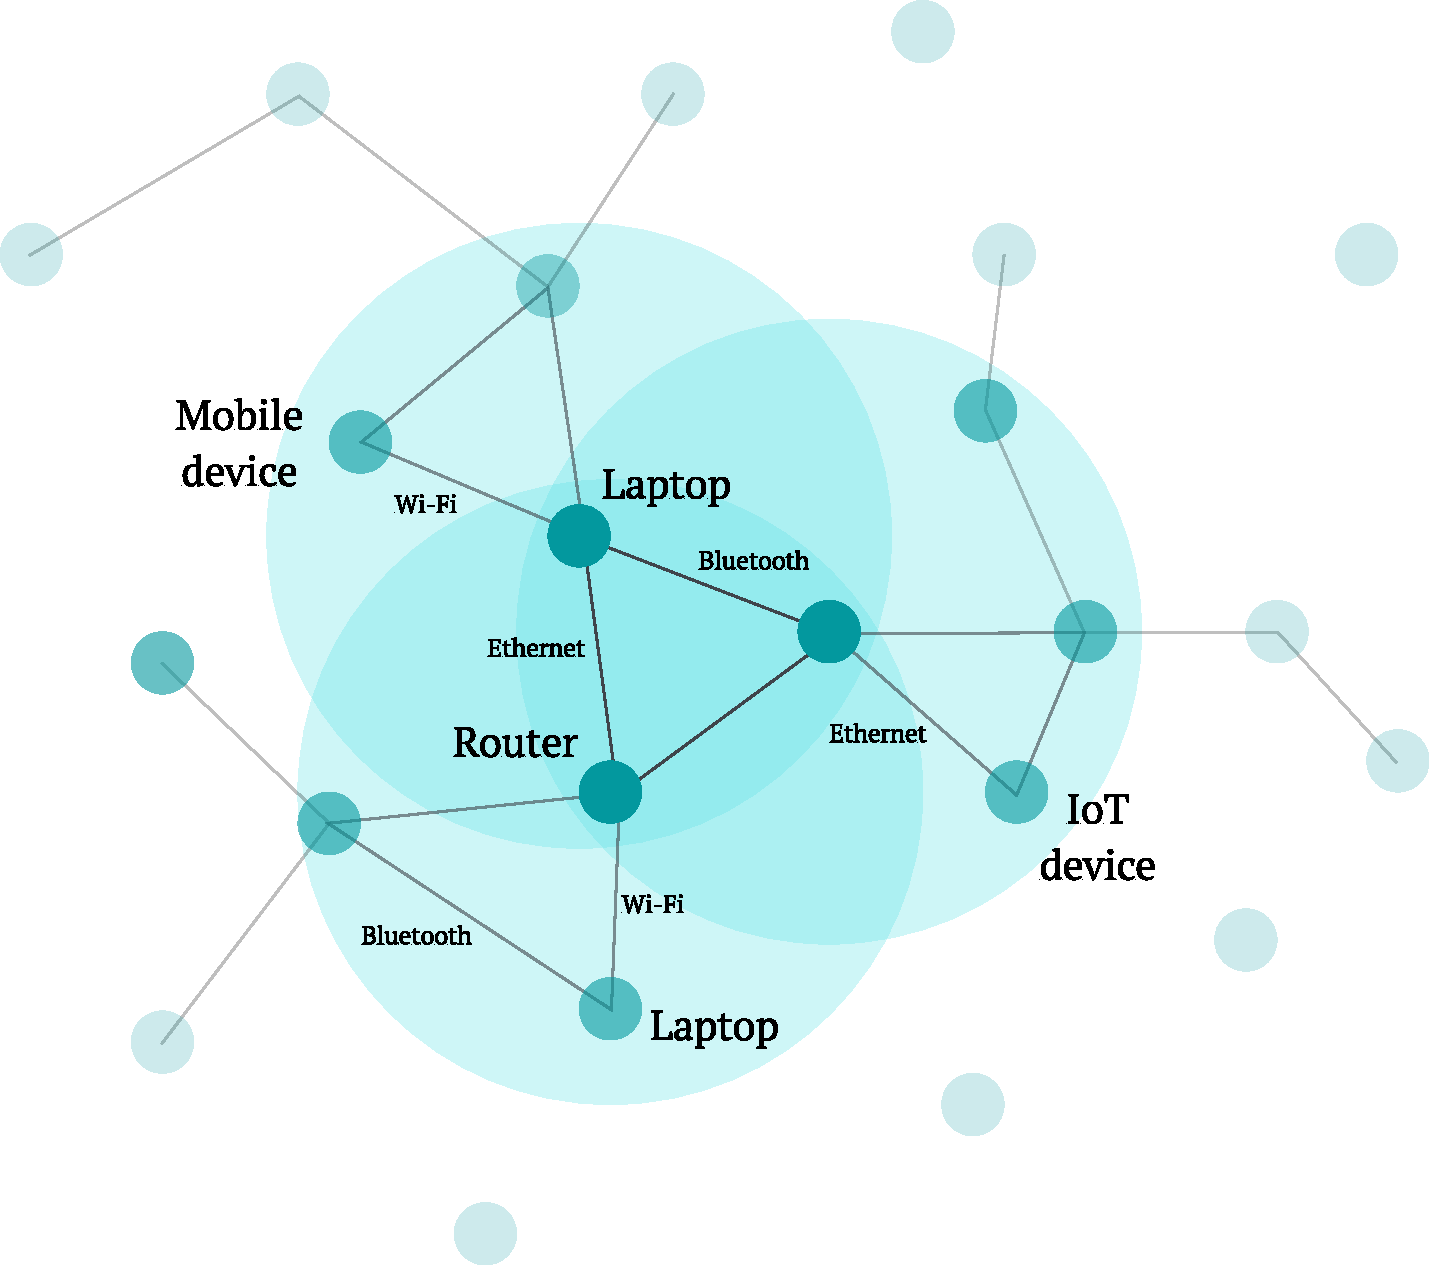
\includegraphics[width=0.65\textwidth]{overview-pol-mesh.pdf}
    \caption{The heterogeneity of a Mesh Network and the substrate diversity of its physical topology~\textemdash~the devices, their connections, and their physical arrangements.}
    \label{fig:proof-of-location-overview-pol-mesh}
    \end{center}
\end{figure}

These routing protocols are expected to operate, not at the network layer, but instead at the data link layer, which is responsible for handling the transmission of data frames over the physical layer. Their main goal is to determine the best path for data frames to travel, based on metrics gathered from lower-level physical information, as, for instance, signal strength and link stability metrics \cite{misra2009guide}. These protocols can support neighbourhood discovery and the ranking of neighbours \cite{batman-adv-v}, and thus potentially enable the processes of zone establishment and zone affinity management, as illustrated in Figure~\ref{fig:proof-of-location-overview-pol-zone-establishment}. Neighbourhood discovery is the process of physically discovering neighbouring nodes within the mesh network \cite{open-mesh-ogmv2}. Neighbour ranking is the process of determining the quality and reliability of each neighbouring link \cite{seither2011routing}. By measuring, understanding, and ranking the quality and reliability of the data links, and by instructing nodes to independently calculate their best next-hops, a routing protocol can establish neighbourhoods and determine the affinity of nodes within these coverage localities. This information can be primarily used to optimize communication paths, reduce congestion, and increase the overall efficiency of the network.

\begin{figure}[h!]
    \begin{center}
    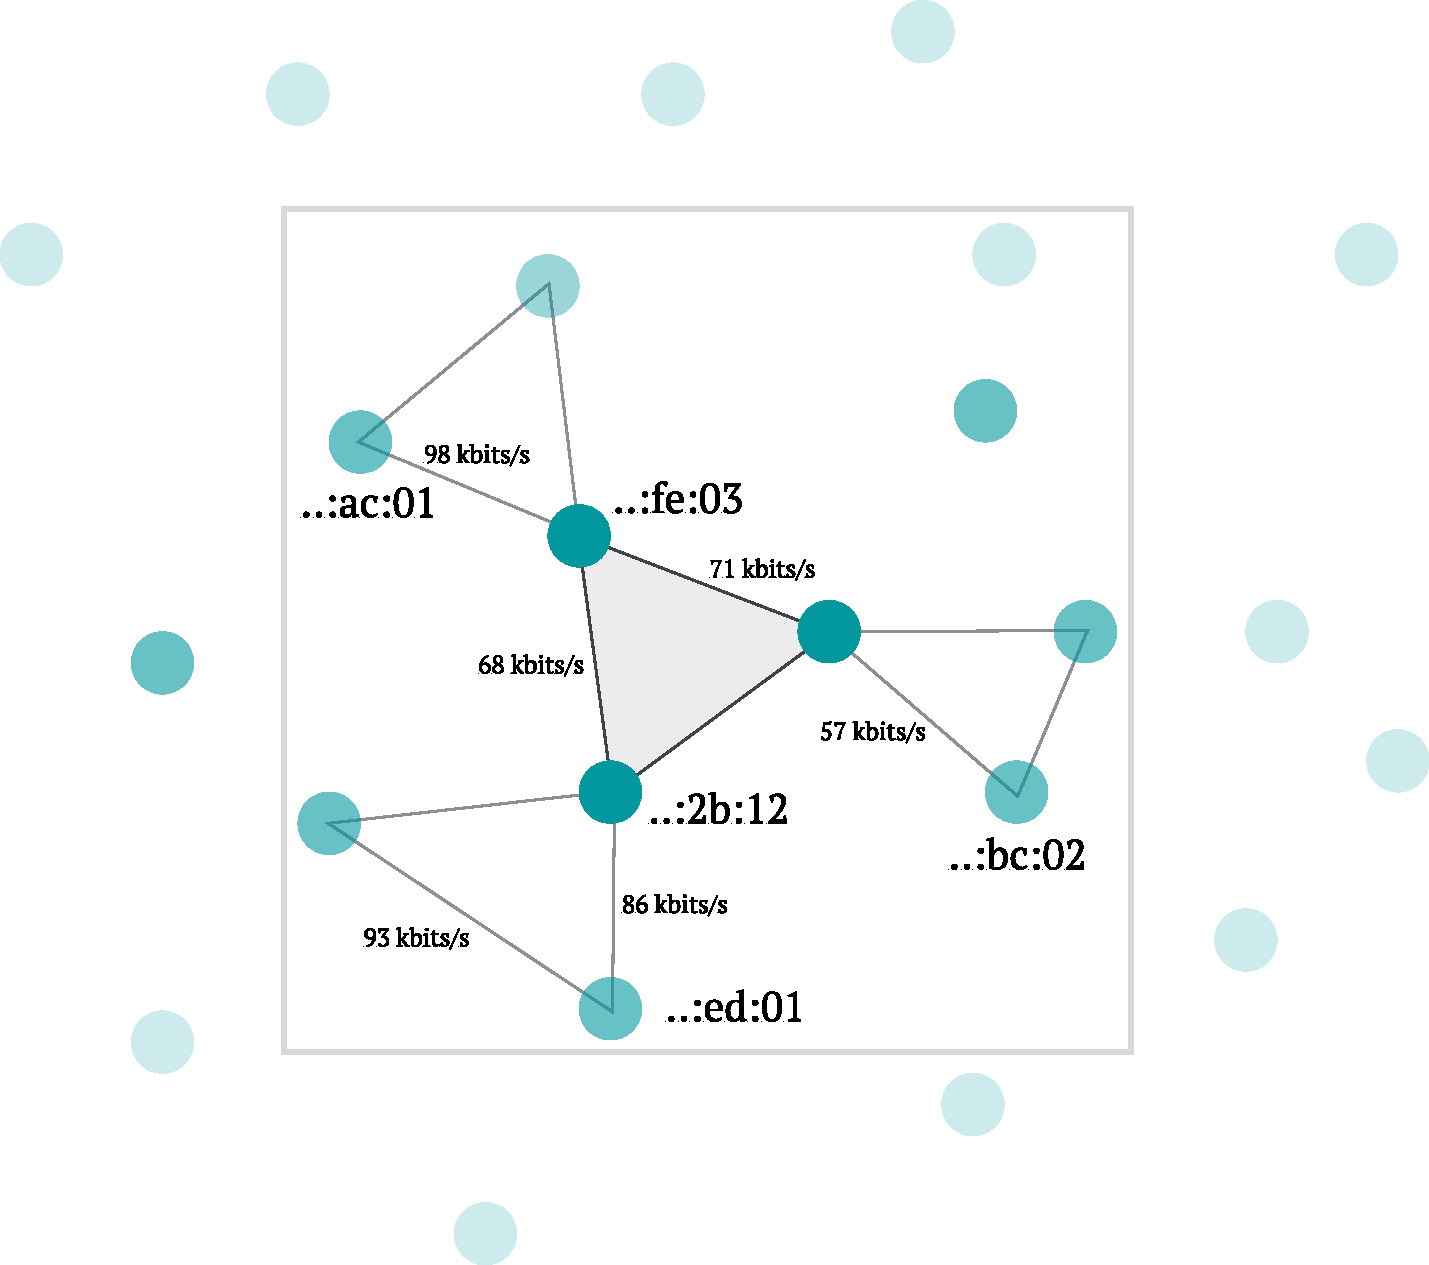
\includegraphics[width=0.7\textwidth]{overview-pol-zone-establishment.pdf}
    \caption{The routing protocol's neighbourhood discovery and ranking processes, using the MAC sublayer and link quality metrics, to enable the establishment of zones within the mesh network.}
    \label{fig:proof-of-location-overview-pol-zone-establishment}
    \end{center}
\end{figure}

The second usage of such accomplishment is to finally enable the targetted establishment of zones within the mesh network. Zones can be viewed as strongly connected sets of neighbours, that, in consequence, are one-hop away from each other. This process of zone establishment is facilitated by the routing protocol, but not strictly enforced, as the protocol solely enables the discovery of potential neighbours and the ranking of their links. The final decision of which nodes are to be grouped together into a zone is left to the nodes themselves, which can then use this information to establish their own zone affinity. Zone affinity is the process of determining the likelihood of nodes communicating and establishing zones with other nodes. The motivation may also be extrinsic to the process of zone discovery or establishment. An identity management protocol, for instance, can be used to determine the zone affinity of nodes, based on their identity and their individual wishes to communicate with other nodes. Incentives of higher degree can be used to motivate nodes to communicate, to establish zones with other relatively specific sets of nodes, and hence to collaborate in the next step of providing zone-relative location services. 
\TODO{Above is too abstract, need example...}
The FOAM protocol, for example, envisions the reliance on token-curated registries to provide a decentralized identity management. It may also rely on crypto-economic incentives to motivate nodes to collaborate and, together, establish and maintain coverage zones, for the higher purpose of providing \pol{} capabilities \cite{foam-white-paper}. This thesis' main focus, with regard to the \poc{} implementation, is abstracted from the whole process of zone establishment and zone affinity management, and assumes that a zone has been already agreed to be established by some out-of-band process. Nonetheless, these aspects are still to be identified for future work, as they are essential for the overall success of the protocol.

After the establishment of operational zones and the affinity filtering potentially happening at the data link layer, the typical Internet Protocol or TCP/IP suite can be used to enable end-to-end data communication for application-specific purposes. The TCP/IP suite consists of a set of protocols that operate at the network and transport layers, providing end-to-end communication services for applications running on different nodes \cite{peterson2007computer}. At the network layer, the Internet Protocol (IP) is used to route data packets within and between the zones, based on their IP addresses. IP is a connectionless protocol that operates independently of the underlying physical and data link layers, allowing it to be used with a variety of network technologies. At the transport layer, protocols such as TCP and UDP can be used to enable end-to-end data communication between application instances. TCP is a reliable, connection-oriented protocol that provides features such as flow control, error detection, and congestion avoidance to ensure that data is transmitted reliably and efficiently between applications. UDP, on the other hand, is a connectionless protocol that provides a lightweight alternative to TCP, suitable for applications that require low-latency communication or do not require reliability guarantees at the transport layer \cite{peterson2007computer}. The choice between the two may be based on the application requirements, the network topology, and the available resources, but the overall conclusion is that, after enabling network layer capabilities, any typical Internet service can be provided to the end-users, sustained by the underlying mesh network. Additionally, as pictured in Figure~\ref{fig:proof-of-location-overview-pol-zone-affinity}, by subnetting and assigning a unique range of IP addresses to each zone, nodes can communicate with each other, in the same zone, and with nodes in other zones using IP-based protocols. Subnetting can also provide a range of benefits, such as improved security, better network management, and more efficient address assignment and usage \cite{peterson2007computer}.

\begin{figure}[h!]
    \begin{center}
    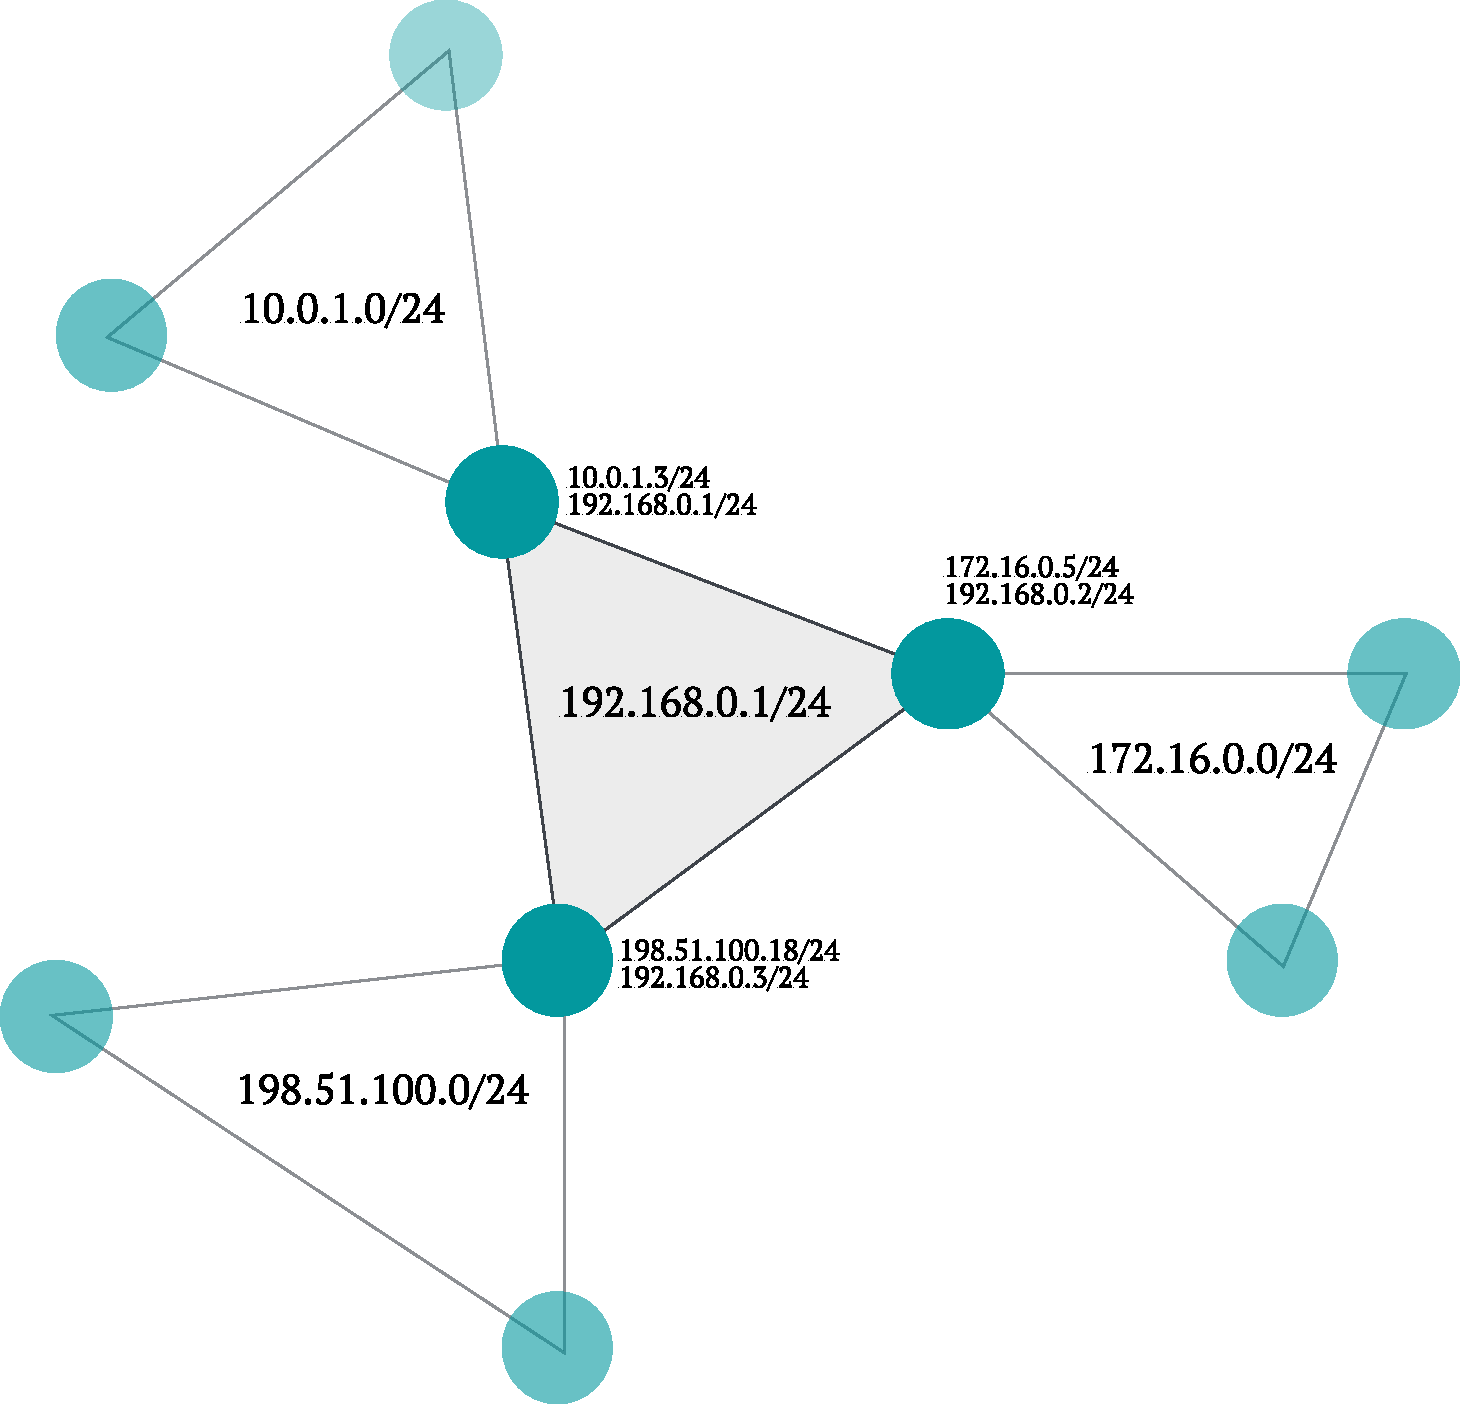
\includegraphics[width=0.6\textwidth]{overview-pol-zone-affinity.pdf}
    \caption{Subnetting and IP-based communication between nodes, within and between zones, after the establishment of their respective zone affinities.}
    \label{fig:proof-of-location-overview-pol-zone-affinity}
    \end{center}
\end{figure}

The following section presents the next step towards guaranteeing the infrastructural basis of the proposed \pol{} protocol, detailing not only the need for zone-relative clock synchronization, but also the steps taken to eventually achieve spatio-temporal soundness. It ultimately assumes that the physical, data link, network, and transport layer capabilities have been already established, and that the nodes are able to communicate with each other using the TCP/IP suite and related protocols, on top of the underlying mesh network infrastructure. The verification or enforcement of the usage of short range communication means is still to be researched, as a key aspect to the protocol's foundational security, and soundness guarantees.

\subsection{Permissionless Consensus} \label{sec:background-permissionless-consensus}

% The following section and subsections reuse the work done in the Distributed Systems Seminar, during the fall semester of the 2022/2023 academic year. The original version of the seminar paper can be found in \cite{units-of-permissionless-consensus}.

Long has been the time when consensus was still on the verge of being considered such a fundamental problem of distributed systems. Generally defined by Lamport et al. \cite{pease1980reaching, lamport2019byzantine}, consensus means reaching an agreement between multiple parties in the potential presence of faulty individuals. As per multi-agent systems, interacting over computer networks, consensus is thought to be the result of a coordination effort, that eventually leads the parties to agree on some value at a given moment. However, the evolution of the consensus problem has been invariably limited by a set of strong assumptions. The well-known Byzantine-Fault-Tolerant multiparty consensus systems, that have been designed over the years, are usually meant to work only with a set of known participants, being them faulty or not \cite{castro1999practical}. 

The other side of the coin is the permissionless consensus challenge, consisting of achieving agreement in an environment where the parties are unknown and untrusted \cite{nakamoto2008bitcoin, buterin2014next}. The relative openness and lack of any kind of central authority are other intrinsic particularities of this type of networks, which inevitably adds complexity to the problem. The participants are not only unknown and untrusted but can also join or leave the network at any time, freely choosing if they care to participate in the consensus protocol. Nevertheless, the problem of permissionless consensus is still seen as a special case of the general consensus definition, but under more meticulous trust assumptions.

Further in this thesis, we will evaluate the different high-level \pol{} protocols and draw a parallel between the evolution of their trust levels and the ultimate need for a low-level permissionless consensus algorithm that allows for establishing decentralized and time-conscious agreement, in an eventual trustless setup, between the multiple witnesses. The next subsections will briefly review some of the most relevant aspects and proof units that give practicality to the roots of the permissionless consensus problem.

\subsubsection{Proof-of-X}

The solution is, nonetheless, unsettled and the scientific community has been reasoning about the need for permissionless consensus when there are already well known and established consensus protocols that work in trusted environments \cite{castro1999practical, miller2016honey}. However, even those protocols have their own limitations, not only in terms of trust, fault-tolerance, centrality, permissions, or bottlenecks, but also in terms of scalability \cite{miller2016honey}, despite assuring deterministic finality \cite{decker2016bitcoin}. The need for permissionless consensus is then justified by the fact that permissioned protocols are not compatible with the requirements of the new generation of distributed systems, especially in the context of Blockchain networks. These requirements include dealing with today's sparse networks of anonymously and dynamically participating devices, without interrupting consensus and while battling the disruption of the system, typically by subverting it with many pseudo-entities~\textemdash~the so-called Sybil attacks \cite{8629877, survey-dist-consensus}. Fundamentally, the permissionless consensus problem is the need for a consensus protocol that can be run in a distributed and decentralized environment, where the participants are unknown and untrusted, and where the network is bigger, sparser and unpredictably less reliable.

Technically, permissionless environments allow for larger networks that depict lower connectivity between the participants. Operationally, everything is expected to happen in an asynchronous or partially synchronous fashion, and the number of transactions is predicted to be smaller than in the permissioned counterparts. Participation is free, and the governance is not centralized, but rather distributed and public. The identity of the participants is secured or semi-secured as it often relies on pseudonymity for protecting the nodes' identity, enabling, at the same time, full transparency concerning the rest of the network's content and operation \cite{xiao2019distributed}. Expectedly, the goal of permissionless consensus, as for any consensus protocol, is to reach agreement on a single value, or a set of values. However, due to the nature of the protocols, the values that are agreed upon end up establishing the serialization of the transactions, and so establishing time consciousness and total order of the events \cite{8629877}.

Also described by Xiao et al. \cite{survey-dist-consensus}, very concisely, the way to achieve an operating protocol, as seen in the mainstream blockchain networks, is by first generating the agreeable value, in this particular case, a block and its proof. Next is the phase of proposing and disseminating the information to the network, followed by the eventual validation and acceptance of the block by the majority of the nodes. This is the approximate moment of probabilistic finality, when consensus is ultimately reached (see Figure~\ref{fig:building-blocks-consensus}). During the whole process, a fair and somewhat predictable incentive mechanism is also needed, that rewards participants for their honest effort in reaching consensus, and punishes the ones that are not behaving correctly. These incentives are of major importance in this very context of permissionless consensus, and all these building phases form the basis of the inner functioning of Bitcoin itself \cite{nakamoto2008bitcoin}, replicated with some variations in other networks \cite{buterin2014next, survey-dist-consensus}. The following section is a short introduction to some relevant proof units that feature in the most popular blockchain systems.

\begin{figure}[h!]
  \begin{center}
  \includegraphics[width=0.9\textwidth]{building-blocks-consensus.pdf}
  \caption{An illustration of the permissionless consensus building phases. From the bottom to the top, the asymmetric arrow of time discretizes the block generation and proposal phases, followed by the block validation, along with frequent network topology changes and the consequent time conscious serialization of the blocks.}
  \label{fig:building-blocks-consensus}
  \end{center}
\end{figure}

\subsubsection{Proof-of-Work and Proof-of-Stake}

Without discrediting the previous attempts, the first practical permissionless consensus algorithm was proposed by Nakamoto in \cite{nakamoto2008bitcoin}. It is a Proof-of-Work consensus protocol that resembles a replicated state machine where the independent participants reach agreement not only about transactional values, but also about their order~\textemdash~naturally forming the underlying structure of what is now known as a blockchain. The focus shifted for decentralized systems and after Proof-of-Work many other consensus mechanisms have been proposed, relying on different consensus units.

In the classical Nakamoto consensus protocol, the generation of a block, to be proposed for further network agreement, complies with the unit of computational work needed to create, or rather find, a verifiable proof of the effort spent on assembling the block \cite{nakamoto2008bitcoin}. This essentially requires brute forcing the search for a cryptographic hash value for the aggregation of the block information with a nonce. This value has to satisfy a difficulty threshold (see Procedure \ref{proc:BlockGeneration}), which gets adjusted dynamically over time, to maintain the network overall requirement for the block generation interval \cite{8629877, survey-dist-consensus}.

\begin{procedure} [!h]
	\caption{BlockGeneration()} \label{proc:BlockGeneration}
	\KwIn{Transaction Merkel Tree Root, Hash of the last Block, Timestamp, Other.}
	\KwResult{new $Block$.}
	\BlankLine
  $BlockHeader \ \gets$ Transaction Merkle Tree Root
  \\ \qquad $| \ $ Hash of the last Block
  \\ \qquad $| \ $ Timestamp
  \\ \qquad $| \ $ Other\;
  \BlankLine
  \tcp{the preceding zero bits in $target$ depict the mining difficulty}
  \While{$Hash(BlockHeader \ | \ nonce) \geq target$}{
    Increment $nonce$\;
  }
  \tcp{append transactional data}
  \Return new $Block$\;
	%\eIf{error messages were found}{\Return \False\;}{\Return \True\;}
\end{procedure}

One can then exercise the reasoning line and extrapolate the previous block generation mechanism to a \emph{Proof-of-Something} pseudo-random competition in which an entity in possession of a higher amount of a certain resource, either computational power, or stake, or certain currency, or, for instance, a higher amount of storage space, guarantees a higher probability of leading the block generation and proposal, consequently winning the acceptance by the majority. This is the essence of Proof-of-Stake, as a derivative of the Proof-of-Work mechanism. Here, stake is a traceable and verifiable amount of a certain unit, token or currency, that is owned by a certain entity who wishes to participate in the consensus protocol. The stake works as a form of collateral that is used to guarantee everyone's honesty, in an attempt to reduce the Sybil attack likelihood. And, respectively as in Proof-of-Work with computational power, the higher the stake, the higher the probability of leading the block generation and proposal.

Idealized and inspired by Proof-of-Stake, extending or adapting Proof-of-Work became a popular trend in the blockchain community. The main idea is to replace the computational power with some other resource, that is more scarce, or more valuable, or more verifiable, or more traceable, to combine multiple resources, or even to add extra requirements to pure Proof-of-Work \cite{survey-dist-consensus}. Not that every one of the options has a considerable potential for entirely solving the permissionless consensus problem, but each one of them may tackle different use cases where consensus needs to be reached, and where different resources are available to make the agreement happen \cite{BOURAGA2021114384, 9376868}. Nonetheless, the design of these consensus mechanisms shall aim for a protocolar choice between a set of properties that form a trilemma: security, scalability, and decentralization. Briefly put, relaxing the security requirements may allow for more scalability, both of which, consequently, have hands tied with decentralization. These trade-offs are of practical consideration when defining the network goals and use cases \cite{survey-dist-consensus}. Further dissection of various classes of Proof-of-Stake based protocols, diverging alternatives to the classic Nakamoto consensus, and comparisons between them can be found in \cite{8629877, survey-dist-consensus, BOURAGA2021114384, 9376868, natoli2019deconstructing}.

With all the above in mind, we will proceed to review some of the proposed \pol{} solutions, discriminated by trust levels. Aiming at achieving spatio-temporal agreement among the witnesses, we will reason about the applicability of one of these permissionless consensus protocols, in the context of a fully decentralized and trustless environment.

\newpage
\section{Related Work} \label{sec:related-work}

This chapter presents a description of the current state of the \pol{} problem, spanning the spectrum of its trust levels, from fully trusted to permissionless environments. Furthermore, it encompasses an assessment of the typical infrastructural scenarios, detailing the progressive shift from centralized to decentralized systems. The organization of the chapter is as follows. Section~\ref{sec:related-work-trusted-centralized} outlines the starting point in a trusted and centralized setting. Section~\ref{sec:related-work-distributed-decentralized} details the progressive shift towards distributed and decentralized protocols. Section~\ref{sec:related-work-fully-trustless} presents the most recent developments in the \pol{} problem, which ultimately target permissionless and fully trustless setups. 

% Finally, alternative strategies to the prevailing \pol{} protocols, which this thesis mainly addresses, are presented in Section~\ref{sec:related-work-alternative-strategies}.


\subsection{Trusted and Centralized Architectures} \label{sec:related-work-trusted-centralized}

The establishment of not just the concept, but also the need for a new kind of systems that, in simple terms, would allow for attesting and prove some device's location, dates back to the early beginnings of this century. 

Waters and Felten, in \cite{waters2003secure}, attempt at pioneering the design of a location-proving system by proximity that simultaneously ensures integrity and privacy. The system model assumes a fully trusted setup, fundamentally composed by two entities, a \emph{verifier} and a \emph{device}. The latter is implicitly thought to be managed by an untrusted user, but hypothesised and expected to be tamper-resistant, and thus trusted by the \emph{verifier}. The motivation behind this scenario is oriented towards practical situations in which, for instance, trusted parties lend their equipment to users and want to verify, or monitor, the equipment's location, such that it remains inside some pre-established location boundaries. The authors explicitly mention the lending of computers by universities and the wish that those devices to not leave the campuses. Home arrest monitoring systems have, as well, the need for ensuring that the ankle device, and so the person in charge, does not escape a certain location. 

Faced with the design and coverage unadaptability of GPS-based location systems, which do not structurally aim at serving as \pol{} enablers, the authors identify the need for small wireless networks, covering a relatively short-ranged area, via a \emph{location manager}, acting as an access point. This \emph{location manager} is either set up, or distinctively trusted by the \emph{verifier}. Round-trip and signal propagation latency are the metrics used, respectively, for determining the proximity of the \emph{device} to the \emph{location manager} and for protecting against proxy attacks~\textemdash~when a proxy device is placed near the \emph{location manager} and serves as signal repeater for the original \emph{device} that is somewhere else, outside the coverage area. Concretely, the work targets Wireless LAN network operators and their existing access points' infrastructure, to serve as \emph{location managers}. A Public Key Infrastructure (PKI) is also proposed in order to delegate the atomic responsibility of authenticating and managing their identities to a trusted third party. Finally, the authors set down the seeds for extending their proximity proof system to a secure and moderately accurate positioning proof mechanism, with the possibility of using multiple \emph{location managers} and a triangulation algorithm.

The \pol{} track was inevitably unfogged with this primordial work and location proofs were soon to be fully demystified and categorically defined. Sariou and Alec, in \cite{saroiu2009enabling}, concisely introduce the primitive concepts around \pol{} and some desired properties of an inherently secure system. However, the key contribution of their work was the delineation of a set of example applications that would benefit from \pol{} protocols. These include, but are not limited to, costumer reward systems for physical stores, location-authenticated business review systems, location-restricted web content delivery, voter's physical presence verification, among many others.

Further protocols took inspiration from this groundwork and started shaping the landscape. Graham and Gray, in \cite{graham2009protecting}, propose a \pol{} scheme called SLVPGP that removes the need for the \emph{location manager} to be trusted by the central \emph{verifier}, delegating the trust to tamper-resistant modules. VeriPlace, by Luo and Hengartner \cite{luo2010veriplace}, is a complex and expensive privacy-aware location proof architecture that distributes responsibility among three types of trusted entities, taking the first step at avoiding dedicated tamper-resistant hardware. It specifically targeted the integration with Yelp\footnote{\url{https://www.yelp.com}}, a public crowd-sourced reviews system for businesses. Another worth mentioning piece of work is from Javali et al. \cite{javali2016alice}, still in a centralized and trusted stand, that adds robustness to the previous protocols by simplifying, in theoretical and practical terms, with trusted and existing Wi-Fi infrastructure, the \pol{} generation process. Finally, the work of Akand et al. \cite{akand2021privacy} is a more recent solidification attempt in the design of centralized but provably secure \pol{} systems that protect against geo-tampering attacks.

The next section will report the emergence of the first relatively distributed \pol{} protocols, taking a step further in the direction of fully decentralized and trustless systems.

\subsection{Progressively Distributed and Decentralized Protocols} \label{sec:related-work-distributed-decentralized}

VeriPlace had already profiled and templated an inherently distributed architecture with built-in privacy awareness, taking a first infrastructural step towards defending against proxy attacks, without the need for trusted hardware \cite{luo2010veriplace}. The whole setup is especially tangled and consequently resourceful for the levels of trust it assumes, but it definitely settled the ground for the next generation of \pol{} schemes. 

\begin{figure}[ht]
    \begin{center}
    \includegraphics[width=0.9\textwidth]{decentralized-pol.pdf}
    \caption{The main arrangements of the APPLAUS protocol, by Zhu and Cao \cite{zhu2011applaus}.}
    \label{fig:decentralized-pol}
    \end{center}
\end{figure}

The following evolutionary stage of these protocols aims at flexing and distributing trust, resources, power, and responsibility, with the hope of achieving more resilient, fault-tolerant, and scalable systems. APPLAUS, by Zhu and Cao \cite{zhu2011applaus}, delivers one of the first distributed protocols that combines the location proof and location privacy problems. It uses Bluetooth enabled mobile devices that communicate with nearby participants, during the proof generation process. The protocol asserts certain bond levels between the \emph{prover}, \emph{verifier}, and \emph{witnesses}, all of them known to a trusted Certificate Authority (CA), disregarding, on the other hand, the need for a fully trusted location proof server to store the historic location records. In Figure~\ref{fig:decentralized-pol}, the essential configuration of the protocol is displayed, envisioning the prover to communicate individually, via Bluetooth, with nearby witnesses. Each witness should agree on providing a location proof, upon the prover's request, to be submitted later to an untrusted location proof server. This server will store the location proof historic records, to be queried by the verifier, in order to assert a prover's location within a specific time period. The prover, witnesses, and verifier are all assumed to be trusted by each other, leaving out the location server. The claim is that, by statistically changing the pseudonyms for each device and by following a user-centric privacy model, the protocol can effectively generate privacy preserving location proofs and store them in a trustless manner. STAMP \cite{wang2016stamp} and PROPS \cite{gambs2014props} are two contemporaneous works that take the same witnessing approach as APPLAUS, but follow the path of convincing the verifier by presenting several shares of a composite location proof, based on group signatures. Both of them try to more profoundly tackle the prover's and witnesses' privacy concerns, but may admittedly fail at preventing collusion scenarios between them. Gambs et al. argue that the reliance on a trusted third party may be an unavoidable requirement, even if against the authors' principles of location sovereignty, especially when one wants to entirely prevent unbounded collusion attacks \cite{gambs2014props}. SPARSE, by Nosouhi et al. \cite{nosouhi2018sparse}, avoids the typical distance-bounding mechanism and the witness picking process by the prover, as done in the previous works, with the goal of protecting against those collusion attempts, at best, in relatively crowded and decentralized witnessing situations. 

At this point, all these schemes have assumed the common goal of protecting the identity of the parties involved in the proof generation process, but they have not yet tackled the additional problem of keeping the location information proportionally private from whoever needs to verify it. Dupin et al. \cite{dupin2018location} theoretically propose a Secure Multi-Party Computation (SMPC) based protocol that is provably resilient against any semi-honest participant. Their solution could still benefit from the classical distance-bounding mechanisms \cite{dupin2018location}, but it is highly resourceful and practically infeasible, since it relies on expensive and complex cryptographic primitives and assumes directional antennas \cite{yang2021group}.

On the horizon of these solutions was still the high level need for detaching \pol{} protocols from any kind of trusted central authority, for both identity and information management. This goal has naturally met, along the way, Blockchain technology. The next section will finally present the most recent developments in achieving decentralized, trustless, and infrastructure-independent \pol{} schemes.


\subsection{Fully Trustless Environments} \label{sec:related-work-fully-trustless}

Inspired by the solution proposed by Zhu and Cao \cite{zhu2011applaus}, Amoretti et al. \cite{amoretti2018blockchain} dive into the definition of a novel decentralized and infrastructure-independent approach that allies together short-range communication technology and Blockchain-based storage and information verification. The authors propose the establishment of a distributed overlay network of linked nodes that, at the same time, wirelessly provide or request location proofs from nearby nodes, and verify or store propagated proofs, via any typical lower-level blockchain protocolar agreement, achieving, thus, permissionless consensus. Their solution is claimed to be one of the very first at protecting against the main location-based-systems' attacks, with the help of a fully decentralized and blockchain inspired peer-to-peer scheme, assuring both integrity and user privacy. Real-world performance evaluation and the possibility for integrating higher-level incentive mechanisms were set as future work prospects. Both Amoretti et al. \cite{amoretti2018blockchain} and Nasrulin et al. \cite{nasrulin2018robust} contemporaneous works illustrate practical constructs that take advantage of the tamper and censorship resistant nature of blockchain technology. The latter tries as well to formalize the main security and spatio-temporal requirements that such a decentralized \pol{} protocol shall present, as seen in Section~\ref{sec:background-proof-of-location}, ending up implementing a \poc{}, based on a permissioned blockchain framework, to specifically solve the challenges related to supply chain tracking.

Further efforts that build upon the above-mentioned solutions are the ones proposed by Wu et al. \cite{wu2020blockchain} and Nosouhi et al. \cite{nosouhi2020blockchain}. The first follows the path of Amoretti et al. \cite{amoretti2018blockchain} and tries to enable, on top of it, user-defined hierarchical privacy protection, with the help of Zero-Knowledge proofs. The proposed protocol finds a bridge between the typical \pol{} set of entities and the usual Zero-Knowledge proof participants. The suggested \emph{zk-PoL} protocol aims at allowing the prover to convince the verifier that one was at a specific location, at a certain point in time, but with a granular privacy preserving disclosure of the location proof details. The obvious motivation of the mechanism is to solve spam, traceability, and privacy concerns of publicly storing raw location information, especially within decentralized and public ledgers. Therefore, the scheme is, to a great degree, centred in the privacy assurances and not in the infrastructural aspects of the potential decentralization that it is built upon. Nevertheless, it sets a promising starting point for the introduction of privacy preserving technology in the realms of trustless \pol{} protocols. Optimizations and faster proof mechanisms are kept in the outlook and waiting to be explored. Nosouhi et al. \cite{nosouhi2020blockchain} stress out a different proximity checking mechanism, to protect against the still unsolved prover and witnesses collusions, while committing, as well, to privacy preserving location proof generation and storage, using public and decentralized blockchain technology. Their work has also an original integration of an incentive mechanism that rewards collaborative participants, in order to more strongly prevent the main known attacks. This sets an unprecedented track for the incorporation of these \pol{} protocols into the digital and decentralized economy that already runs, via Smart Contracts, on blockchain networks like Ethereum \cite{nosouhi2020blockchain, buterin2014next}. 

Minding all the above, Pournaras \cite{pournaras2020proof} proposes the complementing concept of Proof-of-Witness-Presence as a key element in an augmented democracy approach to smart city development. This concept involves validating the accuracy of data collected through participatory crowd-sensing, by requiring physical presence at locations of interest. The author argues that this approach can foster greater citizen engagement and participation in public spaces, and can be incentivized through blockchain consensus and a crypto-economic design. Acknowledging the limitations of current localization methods, such as GPS, it is suggested the need for more advanced and secure location certificates, based on complex social proofs. The Proof-of-Witness-Presence model envisioned by Pournaras may rely on token curated registries and a supplemental fully trustless \pol{} protocol that, for instance, FOAM\footnote{\url{https://foam.space/}} tries to deliver. The next paragraph will be fully dedicated to this last piece of work.

The theorization of the singularity of a four-dimensional manifold, combining the three dimensions of space with the asymmetric arrow of time, has fundamentally shaped humankind's understanding of physical reality. The establishment of an absolute quorum over space and time is the ultimate goal that has driven forward the development of modern globalization, by the way we coordinate and synchronize our existence. Since the institution of the canonical time, sailing through the acknowledgment of the Longitude problem, to finally setting up intercontinental time synchronizers, the absence, or maintenance impossibilities of a truly global and absolute clock is still a major drawback in the production of correct, tamper-resistant, and spatio-temporally sound location information. Asserting the fundamentality of time synchronization, FOAM leverages Einstein's relativity hypothesis to create a new means for measuring space and time, for cartography and map making \cite{king_2020}. Their protocol, combined with their attempt at standardizing location data, is a totally new conceptual way of achieving decentralized, privacy preserving, highly accurate, censorship resistant, verifiable, and secure \pol{}. \emph{Zone Anchors} and \emph{Zone Authorities} form a dynamic and decentralized network of radio beacons and gateways that reach consensus over the precise time of their clocks, establishing zone-relative clock synchronization. This allows for the formation of time conscious zones of witnesses that can simultaneously determine spacial arrangements and provide presence claims. Figure~\ref{fig:trustless-pol} depicts the expectation that Zone Anchors or Zone Authorities dynamically synchronize their internal clocks, establishing a smart contract's enforced physical coverage zone that offers trustless, but spatio-temporally sound location services. Zones may provide precise, verifiable, and secure \pol{} claims, with the precision determined by possible triangulation mechanisms. Combined with token curated registries and crypto-economic incentives, for the maintenance and growth of the decentralized infrastructure, FOAM ultimately aims at creating a global consensus-driven map of the world. Their hopes are on Low Power Wide Area Network (LPWAN) radio technology, for the communication means, and on Ethereum-based Smart Contracts, for decentralized verification, consumption, and incentivization of the protocol operations over the location data \cite{foam-white-paper}.

\begin{figure}[ht]
    \begin{center}
    \includegraphics[width=0.9\textwidth]{trustless-pol.pdf}
    \caption{The FOAM protocol for dynamic and decentralized \pol{} \cite{foam-white-paper}.}
    \label{fig:trustless-pol}
    \end{center}
\end{figure}

The FOAM protocol is the ultimate inspiration for the work developed further in this thesis. The processes of zone establishment, spatio-temporal synchronization, and decentralized witnessing consensus will be explored as in FOAM, but taking advantage of WiFi-based mesh networking for the wireless exchange of information, as introduced in Sections~\ref{sec:background-wireless-mesh-networks}~and~\ref{sec:background-permissionless-consensus}.

% \subsection{Alternative Strategies} \label{sec:related-work-alternative-strategies}

% Inspired by the solution proposed by Zhu and Cao \cite{zhu2011applaus}, Amoretti et al. \cite{amoretti2018blockchain} dive into the definition of a novel decentralized and infrastructure-independent approach that allies together short-range communication technology and Blockchain-based storage and information verification. The authors propose the establishment of a distributed overlay network of linked nodes that, at the same time, wirelessly provide or request location proofs from nearby nodes, and verify or store propagated proofs, via any typical lower-level blockchain protocolar agreement, achieving, thus, permissionless consensus. Their solution is claimed to be one of the very first at protecting against the main location-based-systems' attacks, with the help of a fully decentralized and blockchain inspired peer-to-peer scheme, assuring both integrity and user privacy. Real-world performance evaluation and the possibility for integrating higher-level incentive mechanisms were set as future work prospects. Both Amoretti et al. \cite{amoretti2018blockchain} and Nasrulin et al. \cite{nasrulin2018robust} contemporaneous works illustrate practical constructs that take advantage of the tamper and censorship resistant nature of blockchain technology. The latter tries as well to formalize the main security and spatio-temporal requirements that such a decentralized \pol{} protocol shall present, as seen in Section~\ref{sec:background-proof-of-location}, ending up implementing a \poc{}, based on a permissioned blockchain framework, to specifically solve the challenges related to supply chain tracking.

Further efforts that build upon the above-mentioned solutions are the ones proposed by Wu et al. \cite{wu2020blockchain} and Nosouhi et al. \cite{nosouhi2020blockchain}. The first follows the path of Amoretti et al. \cite{amoretti2018blockchain} and tries to enable, on top of it, user-defined hierarchical privacy protection, with the help of Zero-Knowledge proofs. The proposed protocol finds a bridge between the typical \pol{} set of entities and the usual Zero-Knowledge proof participants. The suggested \emph{zk-PoL} protocol aims at allowing the prover to convince the verifier that one was at a specific location, at a certain point in time, but with a granular privacy preserving disclosure of the location proof details. The obvious motivation of the mechanism is to solve spam, traceability, and privacy concerns of publicly storing raw location information, especially within decentralized and public ledgers. Therefore, the scheme is, to a great degree, centred in the privacy assurances and not in the infrastructural aspects of the potential decentralization that it is built upon. Nevertheless, it sets a promising starting point for the introduction of privacy preserving technology in the realms of trustless \pol{} protocols. Optimizations and faster proof mechanisms are kept in the outlook and waiting to be explored. Nosouhi et al. \cite{nosouhi2020blockchain} stress out a different proximity checking mechanism, to protect against the still unsolved prover and witnesses collusions, while committing, as well, to privacy preserving location proof generation and storage, using public and decentralized blockchain technology. Their work has also an original integration of an incentive mechanism that rewards collaborative participants, in order to more strongly prevent the main known attacks. This sets an unprecedented track for the incorporation of these \pol{} protocols into the digital and decentralized economy that already runs, via Smart Contracts, on blockchain networks like Ethereum \cite{nosouhi2020blockchain, buterin2014next}. 

Minding all the above, Pournaras \cite{pournaras2020proof} proposes the complementing concept of Proof-of-Witness-Presence as a key element in an augmented democracy approach to smart city development. This concept involves validating the accuracy of data collected through participatory crowd-sensing, by requiring physical presence at locations of interest. The author argues that this approach can foster greater citizen engagement and participation in public spaces, and can be incentivized through blockchain consensus and a crypto-economic design. Acknowledging the limitations of current localization methods, such as GPS, it is suggested the need for more advanced and secure location certificates, based on complex social proofs. The Proof-of-Witness-Presence model envisioned by Pournaras may rely on token curated registries and a supplemental fully trustless \pol{} protocol that, for instance, FOAM\footnote{\url{https://foam.space/}} tries to deliver. The next paragraph will be fully dedicated to this last piece of work.

The theorization of the singularity of a four-dimensional manifold, combining the three dimensions of space with the asymmetric arrow of time, has fundamentally shaped humankind's understanding of physical reality. The establishment of an absolute quorum over space and time is the ultimate goal that has driven forward the development of modern globalization, by the way we coordinate and synchronize our existence. Since the institution of the canonical time, sailing through the acknowledgment of the Longitude problem, to finally setting up intercontinental time synchronizers, the absence, or maintenance impossibilities of a truly global and absolute clock is still a major drawback in the production of correct, tamper-resistant, and spatio-temporally sound location information. Asserting the fundamentality of time synchronization, FOAM leverages Einstein's relativity hypothesis to create a new means for measuring space and time, for cartography and map making \cite{king_2020}. Their protocol, combined with their attempt at standardizing location data, is a totally new conceptual way of achieving decentralized, privacy preserving, highly accurate, censorship resistant, verifiable, and secure \pol{}. \emph{Zone Anchors} and \emph{Zone Authorities} form a dynamic and decentralized network of radio beacons and gateways that reach consensus over the precise time of their clocks, establishing zone-relative clock synchronization. This allows for the formation of time conscious zones of witnesses that can simultaneously determine spacial arrangements and provide presence claims. Figure~\ref{fig:trustless-pol} depicts the expectation that Zone Anchors or Zone Authorities dynamically synchronize their internal clocks, establishing a smart contract's enforced physical coverage zone that offers trustless, but spatio-temporally sound location services. Zones may provide precise, verifiable, and secure \pol{} claims, with the precision determined by possible triangulation mechanisms. Combined with token curated registries and crypto-economic incentives, for the maintenance and growth of the decentralized infrastructure, FOAM ultimately aims at creating a global consensus-driven map of the world. Their hopes are on Low Power Wide Area Network (LPWAN) radio technology, for the communication means, and on Ethereum-based Smart Contracts, for decentralized verification, consumption, and incentivization of the protocol operations over the location data \cite{foam-white-paper}.

\begin{figure}[ht]
    \begin{center}
    \includegraphics[width=0.9\textwidth]{trustless-pol.pdf}
    \caption{The FOAM protocol for dynamic and decentralized \pol{} \cite{foam-white-paper}.}
    \label{fig:trustless-pol}
    \end{center}
\end{figure}

The FOAM protocol is the ultimate inspiration for the work developed further in this thesis. The processes of zone establishment, spatio-temporal synchronization, and decentralized witnessing consensus will be explored as in FOAM, but taking advantage of WiFi-based mesh networking for the wireless exchange of information, as introduced in Sections~\ref{sec:background-wireless-mesh-networks}~and~\ref{sec:background-permissionless-consensus}.

\newpage
\section{Protocol Fundamentals} \label{sec:protocol-fundamentals}

This section outlines the key requirements and long-term goals of the proposed \pol{} protocol, as well as a detailed scenario that illustrates how such a system may function in a real-world context. It also provides a comprehensive overview of the thesis' objectives, while aiming at contextualizing the subsequent technical development work.

\subsection{Overview} \label{sec:protocol-fundamentals-overview}

The general approach to the design of \pol{} protocols has been mainly focused on the proof generation process, as seen in the multiple examples dissected in Chapter~\ref{sec:related-work}. Advancements made towards more distributed and decentralized solutions have highlighted the need for a comprehensive and detailed description of the protocol's entire range of requirements. To achieve an operable system that meets the demands of real-world applications, a phased strategy with a keen awareness of the intrinsic details, at every stage of the solution, is essential for providing a complete and coherent picture of the protocol's design. Therefore, we will attempt at the design of a \pol{} protocol that starts with an infrastructural foundation, and ends with a complete system~\textemdash~aiming to achieve the goal of proving one's location.

\begin{figure}[ht]
    \begin{center}
    \includegraphics[width=0.9\textwidth]{overview-pol.pdf}
    \caption{A discretization attempt to capture the multiple steps of the protocol design, from a dynamic mesh topology, towards the ultimate goal of achieving Absolute \pol.}
    \label{fig:proof-of-location-overview}
    \end{center}
\end{figure}

The following sections will guide the reader through the multiple steps of the protocol's design. This journey, depicted in Figure~\ref{fig:proof-of-location-overview}, starts with the understructure of the system, powered by a dynamic and non-hierarchic Mesh Network topology. This topology should enable the network agents to communicate with each other in a peer-to-peer, short-ranged, and conveniently wireless fashion. The next step entails the nodes' neighbourhood establishment, eased by lower-layer routing protocols, leading to the eventual creation of fully connected zones of neighbours. Each node, however, may simultaneously belong to multiple zones, with the processes of zone affinity, zone switching, zone expanding, and, consequently, the overall configuration of the mesh topology being dictated by protocolar arrangements, or even, application level incentives. The theoretical aim is at achieving a latticework of space and time, with zone-relative clock precision. Therefore, the next step is to establish, or derive, spatio-temporal zone synchronization. Space synchrony is achieved with the assumptions regarding the short-ranged communication means. Time synchrony requires a clock synchronization mechanism, which may simultaneously allow for zone-relative event serialization, via a Turing-complete strongly consistent consensus-based system. Nonetheless, the main aim is to achieve zone-relative time consciousness, to finally enable spatio-temporal soundness \cite{nasrulin2018robust}.

In the following sections, we provide a more detailed analysis of these multiple steps, but will point only, in practical terms, to a subset of the entire problem. The steps that precede the zone discovery and zone affinity procedures, as well as the ones that succeed the goal of achieving relative \pol{} are either abstracted, explicitly assumed, or left for future work.

% \TODO{Should it be called "Zone Establishment"? Or rather "Zone Discovery"? Read the next section for more details... But keep this question in mind to decide what makes more sense}

\subsection{Dynamic and Non-Hierarchic Mesh Networks} \label{sec:protocol-fundamentals-mesh}

Dynamic and non-hierarchic mesh networks are a type of wireless network architecture that allows for the creation of ad hoc networks in which nodes can communicate with each other without the need for a central coordinating device. This type of network is characterized by its ability to self-organize and dynamically adapt to both changes in the environment and in the overall network topology. As presented in Section~\ref{sec:background-wireless-mesh-networks}, one of the key features that materializes the concept of dynamic and non-hierarchic mesh networks is the existence and implementation of lower-layer routing protocols to facilitate the peer-to-peer communication between the nodes.

Mesh networks, as expected, rely first on the physical layer, according to the standards of computer networking, which is responsible for transmitting raw bit stream data over the physical medium, copper wire, optical fibre, or wireless frequencies, for example. This layer defines the physical characteristics of the data transmission, such as voltage levels, data rates, and the physical connectors and media used for communication. Its main function is to provide a reliable and efficient transmission of bits between devices, without any regard made to the higher-layer protocols and their associated data. The physical layer is responsible for encoding and decoding data into a format that can be transmitted over the network, while also detecting and correcting errors that occur during transmission \cite{peterson2007computer}. It also defines the substrate physical topology of the network, which describes the arrangement of the physical components such as devices, cables, and other network equipment, as depicted in Figure~\ref{fig:proof-of-location-overview-pol-mesh}. To then enable efficient and coordinated communication, there is a need for routing protocols that determine the best path for data packets to travel through.

\begin{figure}[h!]
    \begin{center}
    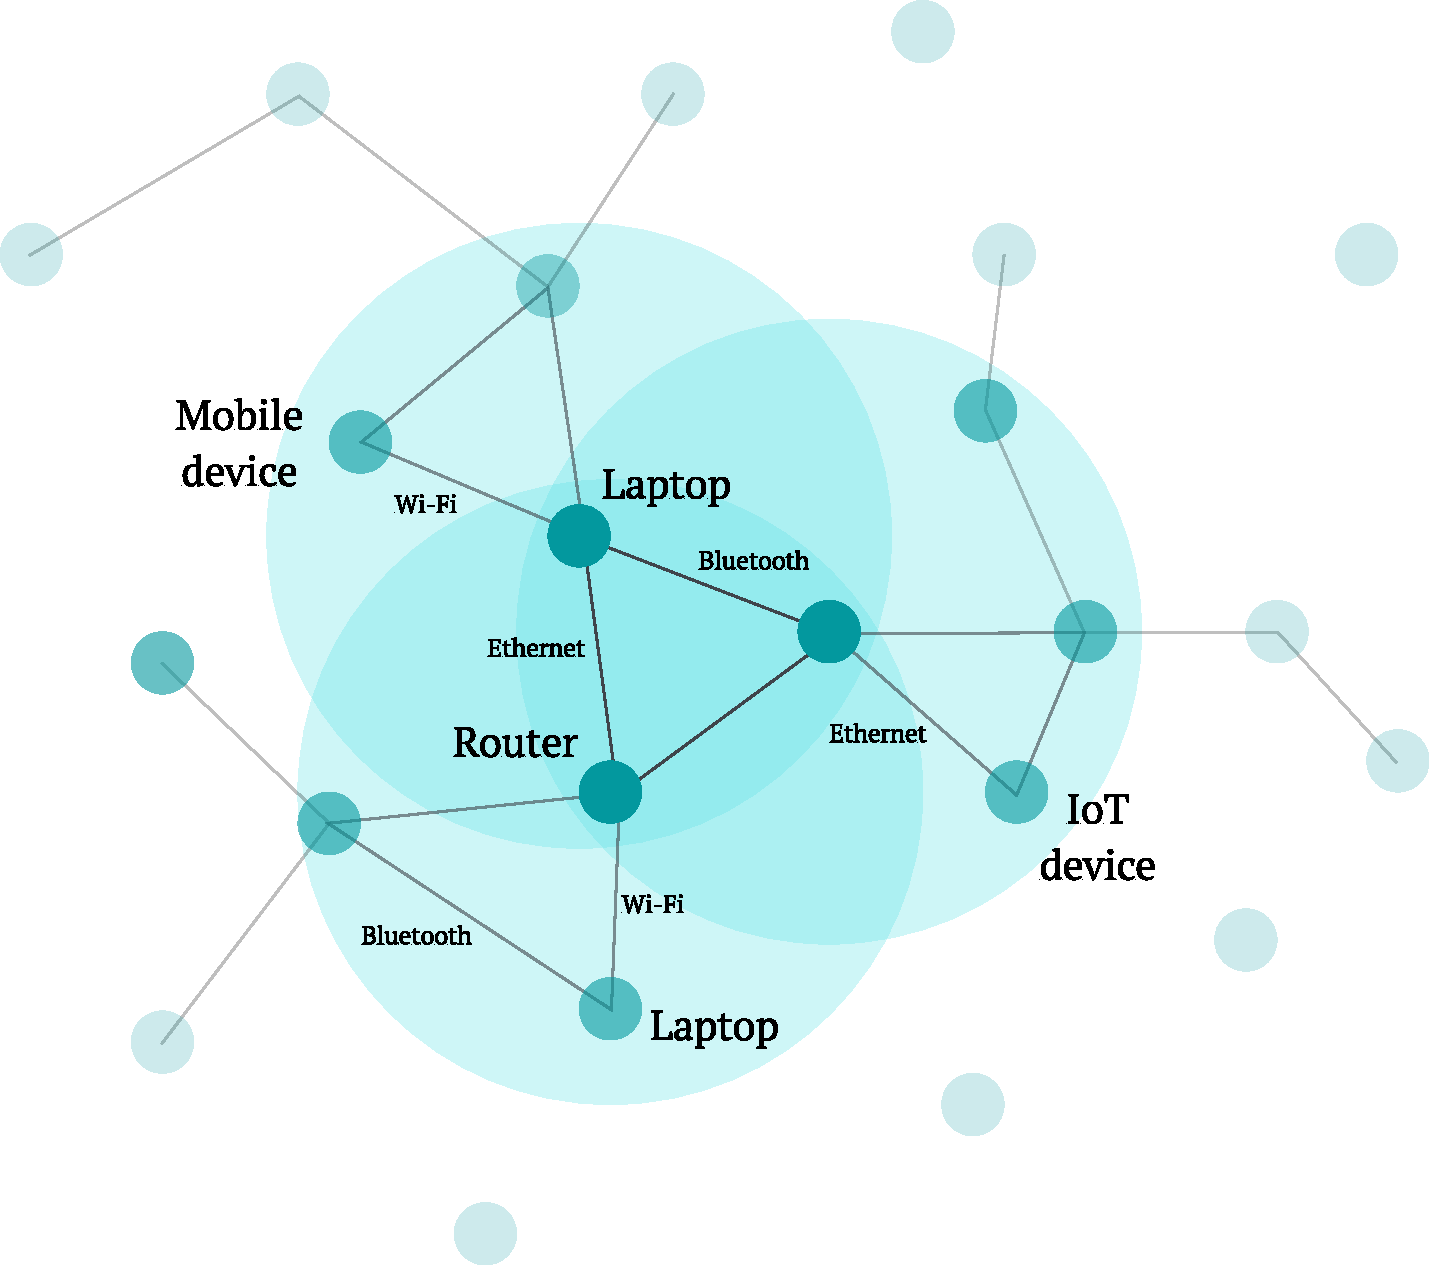
\includegraphics[width=0.65\textwidth]{overview-pol-mesh.pdf}
    \caption{The heterogeneity of a Mesh Network and the substrate diversity of its physical topology~\textemdash~the devices, their connections, and their physical arrangements.}
    \label{fig:proof-of-location-overview-pol-mesh}
    \end{center}
\end{figure}

These routing protocols are expected to operate, not at the network layer, but instead at the data link layer, which is responsible for handling the transmission of data frames over the physical layer. Their main goal is to determine the best path for data frames to travel, based on metrics gathered from lower-level physical information, as, for instance, signal strength and link stability metrics \cite{misra2009guide}. These protocols can support neighbourhood discovery and the ranking of neighbours \cite{batman-adv-v}, and thus potentially enable the processes of zone establishment and zone affinity management, as illustrated in Figure~\ref{fig:proof-of-location-overview-pol-zone-establishment}. Neighbourhood discovery is the process of physically discovering neighbouring nodes within the mesh network \cite{open-mesh-ogmv2}. Neighbour ranking is the process of determining the quality and reliability of each neighbouring link \cite{seither2011routing}. By measuring, understanding, and ranking the quality and reliability of the data links, and by instructing nodes to independently calculate their best next-hops, a routing protocol can establish neighbourhoods and determine the affinity of nodes within these coverage localities. This information can be primarily used to optimize communication paths, reduce congestion, and increase the overall efficiency of the network.

\begin{figure}[h!]
    \begin{center}
    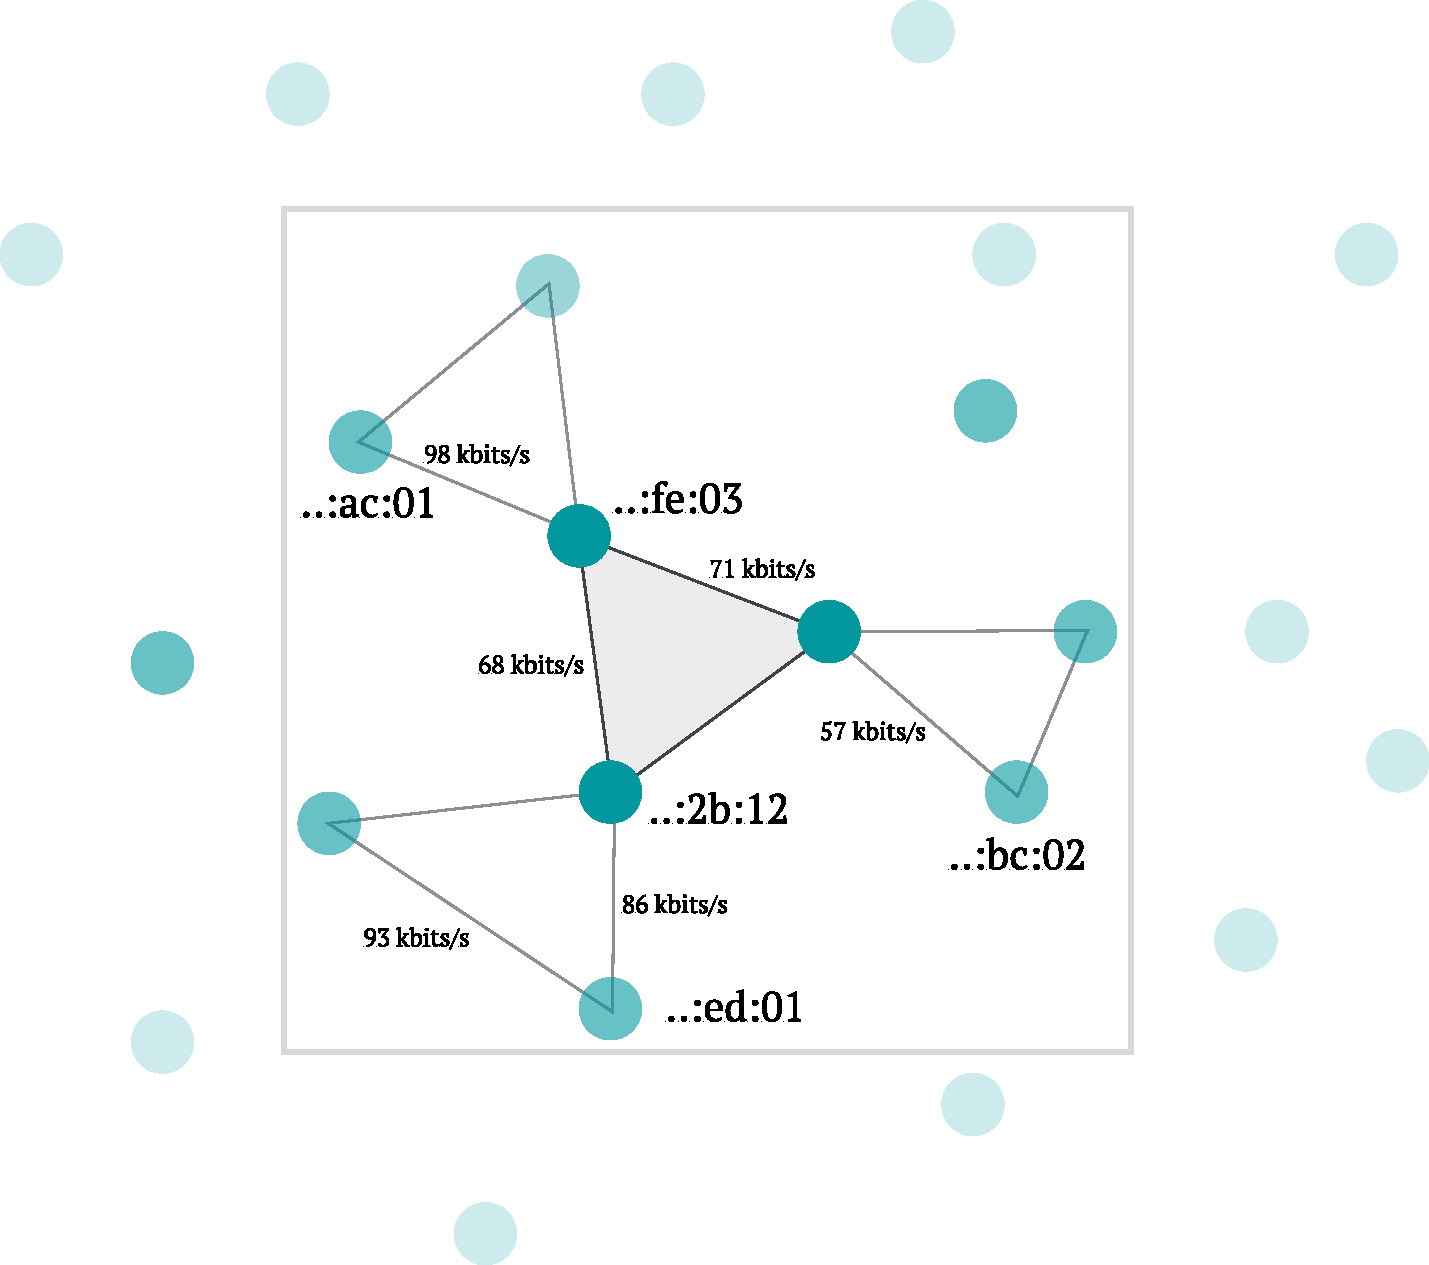
\includegraphics[width=0.7\textwidth]{overview-pol-zone-establishment.pdf}
    \caption{The routing protocol's neighbourhood discovery and ranking processes, using the MAC sublayer and link quality metrics, to enable the establishment of zones within the mesh network.}
    \label{fig:proof-of-location-overview-pol-zone-establishment}
    \end{center}
\end{figure}

The second usage of such accomplishment is to finally enable the targetted establishment of zones within the mesh network. Zones can be viewed as strongly connected sets of neighbours, that, in consequence, are one-hop away from each other. This process of zone establishment is facilitated by the routing protocol, but not strictly enforced, as the protocol solely enables the discovery of potential neighbours and the ranking of their links. The final decision of which nodes are to be grouped together into a zone is left to the nodes themselves, which can then use this information to establish their own zone affinity. Zone affinity is the process of determining the likelihood of nodes communicating and establishing zones with other nodes. The motivation may also be extrinsic to the process of zone discovery or establishment. An identity management protocol, for instance, can be used to determine the zone affinity of nodes, based on their identity and their individual wishes to communicate with other nodes. Incentives of higher degree can be used to motivate nodes to communicate, to establish zones with other relatively specific sets of nodes, and hence to collaborate in the next step of providing zone-relative location services. 
\TODO{Above is too abstract, need example...}
The FOAM protocol, for example, envisions the reliance on token-curated registries to provide a decentralized identity management. It may also rely on crypto-economic incentives to motivate nodes to collaborate and, together, establish and maintain coverage zones, for the higher purpose of providing \pol{} capabilities \cite{foam-white-paper}. This thesis' main focus, with regard to the \poc{} implementation, is abstracted from the whole process of zone establishment and zone affinity management, and assumes that a zone has been already agreed to be established by some out-of-band process. Nonetheless, these aspects are still to be identified for future work, as they are essential for the overall success of the protocol.

After the establishment of operational zones and the affinity filtering potentially happening at the data link layer, the typical Internet Protocol or TCP/IP suite can be used to enable end-to-end data communication for application-specific purposes. The TCP/IP suite consists of a set of protocols that operate at the network and transport layers, providing end-to-end communication services for applications running on different nodes \cite{peterson2007computer}. At the network layer, the Internet Protocol (IP) is used to route data packets within and between the zones, based on their IP addresses. IP is a connectionless protocol that operates independently of the underlying physical and data link layers, allowing it to be used with a variety of network technologies. At the transport layer, protocols such as TCP and UDP can be used to enable end-to-end data communication between application instances. TCP is a reliable, connection-oriented protocol that provides features such as flow control, error detection, and congestion avoidance to ensure that data is transmitted reliably and efficiently between applications. UDP, on the other hand, is a connectionless protocol that provides a lightweight alternative to TCP, suitable for applications that require low-latency communication or do not require reliability guarantees at the transport layer \cite{peterson2007computer}. The choice between the two may be based on the application requirements, the network topology, and the available resources, but the overall conclusion is that, after enabling network layer capabilities, any typical Internet service can be provided to the end-users, sustained by the underlying mesh network. Additionally, as pictured in Figure~\ref{fig:proof-of-location-overview-pol-zone-affinity}, by subnetting and assigning a unique range of IP addresses to each zone, nodes can communicate with each other, in the same zone, and with nodes in other zones using IP-based protocols. Subnetting can also provide a range of benefits, such as improved security, better network management, and more efficient address assignment and usage \cite{peterson2007computer}.

\begin{figure}[h!]
    \begin{center}
    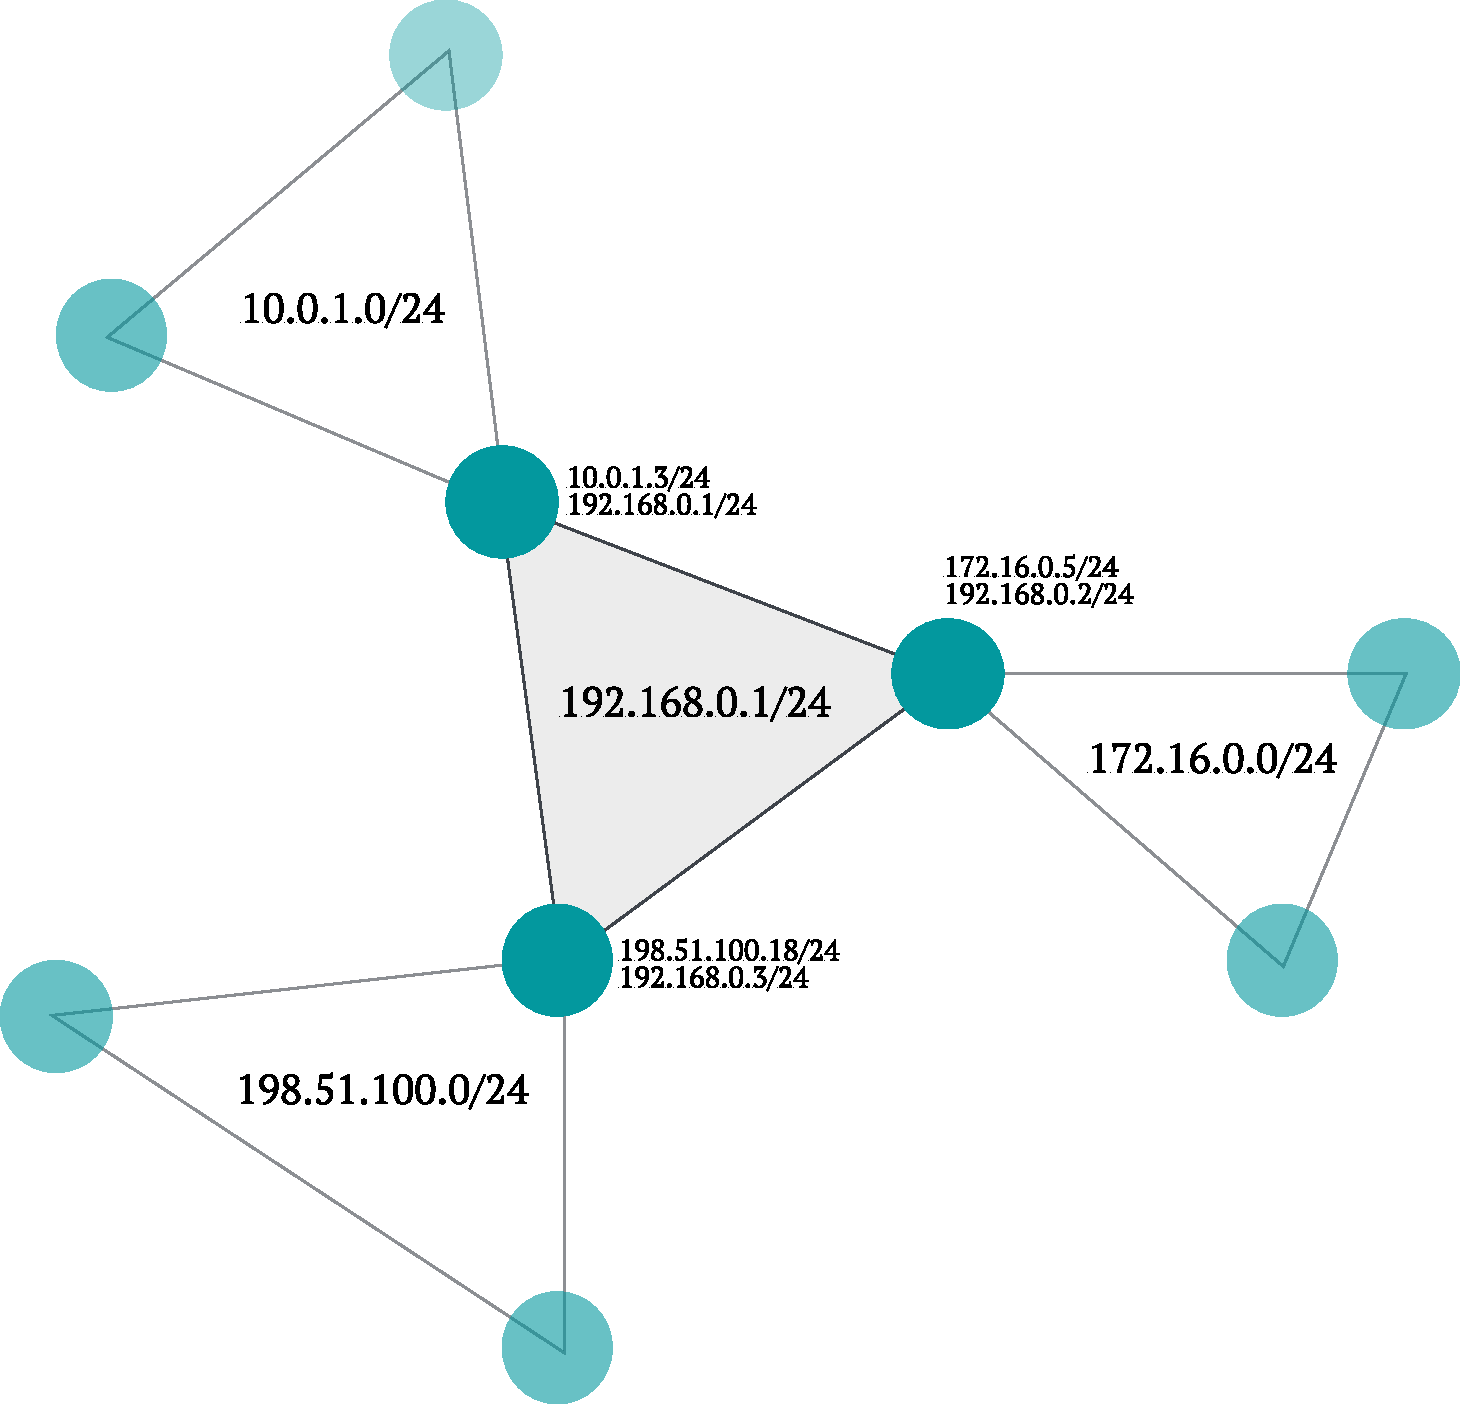
\includegraphics[width=0.6\textwidth]{overview-pol-zone-affinity.pdf}
    \caption{Subnetting and IP-based communication between nodes, within and between zones, after the establishment of their respective zone affinities.}
    \label{fig:proof-of-location-overview-pol-zone-affinity}
    \end{center}
\end{figure}

The following section presents the next step towards guaranteeing the infrastructural basis of the proposed \pol{} protocol, detailing not only the need for zone-relative clock synchronization, but also the steps taken to eventually achieve spatio-temporal soundness. It ultimately assumes that the physical, data link, network, and transport layer capabilities have been already established, and that the nodes are able to communicate with each other using the TCP/IP suite and related protocols, on top of the underlying mesh network infrastructure. The verification or enforcement of the usage of short range communication means is still to be researched, as a key aspect to the protocol's foundational security, and soundness guarantees.

\subsection{Turing-Complete Clock Synchronization} \label{sec:protocol-fundamentals-clock}

Section~\ref{sec:related-work-fully-trustless} has already outlined the invariable need for clock synchronization, when it comes to reach progressively more accurate, correct, sound, and tamper-proof means of location attestation. What has not been discussed yet is the bridge between the clock synchronization problem and the consensus problem, in the specific context of distributed systems. 

This section will briefly discuss how these two fundamental problems are, in fact, intertwined. In simple terms, synchronizing clocks is nothing more profound than reaching agreement about the current time of the internal clocks of a distributed setting of machines. The indiscriminate case of clock synchronization can be stretched to a continued act of counting time at the same pace, as the indiscriminate case of reaching agreement about the current time of the internal clocks can be extended to a continued act of reaching agreement about the current state of the system. The latter is the consensus problem, and the former is a special case of it, the case of time synchronization. As argued in Section~\ref{sec:background-permissionless-consensus}, craving to achieve time synchronization, in not just a distributed setting, but in a fully trustless environment, can be transposed to the problem of achieving permissionless consensus, fulfilling the need for ordering and synchronizing events, at the same pace, in an environment where individual participants are not necessarily trusted. The first example depicted in Figure~\ref{fig:proof-of-location-example-scenarios} makes it clear that the eyewitnesses can only attest to the reporter's presence at the accident site if they had been there at the same time and witnessed the same event. However, these entities are not necessarily known to each other and to anyone else around, nor are they necessarily trusted. This implies not trusting that the clocks of the witnesses are correctly adjusted, as well. Therefore, the witnesses need to reach agreement about the current time, in order to be able to collectively and correctly attest to the reporter's presence at the accident site, in a given moment, otherwise they would all have conflicting or different reports. Additional to that, they may also attest to the reporter's course of action, by the means of taking pictures or recording videos, which are also events that may be ordered and synchronized, achieving, thus, permissionless consensus.

In consequence and specifically regarding the \pol{} problem, the need for clock synchronization is not only a matter of achieving more accurate positioning measures, as typically done in GPS-related trilateration systems, but a fundamental matter of achieving complete and sound consensus between the witnesses that are set to attest to one's location. Fundamentally, as defined in Section~\ref{sec:background-proof-of-location}, a \pol{} is complete if the attestation is done at location $l$ and time $t$, by a set of witnesses $w \in W$. To cope, as well, with the proposed property of spatio-temporal soundness, these witnesses should invariably reach consensus. They should not just agree to exist at around the same location $l$, relative to the precision, reliability, and coverage of their physical communication means, but should also agree on the time $t$, relative to the precision of their internal clocks. The latter is exactly the clock synchronization problem, folded into the greater and abstract need for consensus. The FOAM protocol proposes the achievement of such a time agreement with the employment of a self-stabilizing hybrid fault-tolerant clock synchronization protocol \cite{foam-white-paper, malekpour2015self}. The authors justify the choice highlighting the formal verification methods employed in Malekpour's work. This distributed algorithm is expected to formally work to the extent of the presence of a one third minority of Byzantine nodes \cite{lamport2019byzantine}. This fact validates the theoretical need for a composition of at least four witnesses for the most basic configuration of a zone, in the FOAM protocol. 

\begin{figure}[b!]
    \begin{center}
    \includegraphics[width=0.8\textwidth]{overview-pol-time-sync.pdf}
    \caption{The goal of establishing zone-relative time consciousness, on the left, by the employment of a clock synchronization protocol, and on the right, by the employment of a consensus mechanism. Relative to the precision of both frequencies, the two mechanisms should achieve the same result, with the latter allowing for a strongly consistent serialization of transactions and total order of multidimensional information.}
    \vspace{-1cm}
    \label{fig:proof-of-location-overview-time-sync}
    \end{center}
\end{figure}

\begin{figure}[b!]
    \begin{center}
    \includegraphics[width=0.6\textwidth]{overview-pol-latticework.pdf}
    \caption{The dense latticework of time-conscious witnessing zones, providing location services. Such a structure would allow for more accurate and verifiable location attestations, for example, regarding moving provers that constantly change their locations.}
    \vspace{-1cm}
    \label{fig:proof-of-location-overview-latticework}
    \end{center}
\end{figure}

This thesis proposes, instead, the empirical experimentation with a permissionless consensus mechanism, in the lines of the ones introduced in Section~\ref{sec:background-permissionless-consensus}. The goal, as illustrated in Figure~\ref{fig:proof-of-location-overview-time-sync}, is equivalent to establishing zone-relative time consciousness, but with the added benefit of providing strongly consistent serialization of transactions and total order of multidimensional events, instead of simply counting time in a unidimensional manner. The technicalities of modern systems that tackle the permissionless consensus problem allow, as well, for stronger guarantees in terms of security, tamper-proof and censorship resistance, as discussed in Section~\ref{sec:related-work-fully-trustless}. The fault-tolerance guarantees of a typical deterministic-finality Byzantine fault-tolerant algorithm are shifted back to a probabilistic finality fault-tolerance threshold, where the probability of a transaction being finalized is directly proportional to the number of nodes that have approved it \cite{survey-dist-consensus}. This is, arguably, a more desirable property for the considerations of a decentralized \pol{} protocol, where the finality of a location certificate is directly proportional to the number of witnesses that have seen the prover, and thus, the number of witnesses that have agreed on the time of the attestation, in the context of trustless environments. The methodical work of formally verifying, measuring, and comparing the two approaches, in the specific context of \pol{} protocols, is also left for future work. This thesis will plainly focus on the experimentation with a consensus mechanism that not only allows for the logical synchronization of clocks, via the regulation of the block interval, an inherent property of such mechanisms, but also for the achievement of a distributed and time-conscious Turing Complete environment, where the execution of more sophisticated logic is structurally enabled, in a decentralized setting. Another point worth mentioning is the extensibility of the proposed way of achieving clock synchronization, which should also be researched further, to assess the need and evaluate the possibility for independently calculating the geometry of the zone, and the practicability of trilateration mechanisms to more accurately determine the prover's exact location \cite{foam-white-paper}. Nevertheless, the theorized approach aligns itself with the spacetime model of a multidimensional manifold and the special relativity idea of a dense latticework of clocks, as depicted in Figure~\ref{fig:proof-of-location-overview-latticework}. The end goal for the coverage expansion of such a \pol{} protocol is to achieve a global latticework of witnessing zones that provide location services. This resonates with the faraway goal of achieving a secure, verifiable, decentralized, global and consensus-driven map of the world \cite{king_2020,foam-white-paper}.

The potential Turing Completeness property of the envisioned consensus system fundamentally allows for a network of nodes to perform arbitrary computations in a decentralized and fault-tolerant manner. At its core and in more tangible terms, such a system allows for the creation of smart contracts, as self-executing code agreements that are dictated by the terms of the direct consensus between the entities that are involved in the \pol{} protocol. By using a distributed Turing-Complete system, like Ethereum \cite{buterin2014next}, these smart contracts can be deployed across the network, and their execution can be verified by all entities, ensuring that the terms of the contract are met. This allows for the simple transactional case of registering a valid \pol{} claim by the prover, which will be covered in this thesis, and also for progressively more complex location claims. Pictured in Figure~\ref{fig:proof-of-location-overview-turing}, a Turing Complete system could, for example, enable a multi-prover configuration, or enforce a set of arbitrary terms dictated by the verifier, the witnesses, or by zone-specific requirements, among all other endless computable possibilities that one may envision. 

\begin{figure}[h!]
    \begin{center}
    \includegraphics[width=0.9\textwidth]{overview-pol-turing.pdf}
    \caption{Some more sophisticated use cases of a Turing Complete \pol{} protocol, where the execution of zone-relative smart contracts is enabled. On the left, a multi-prover configuration, where the witnesses are required to attest to the simultaneous existence of a group of provers, and on the right, the case where a verifier enforces the attestation of the prover's location at a specific block, or time.}
    \label{fig:proof-of-location-overview-turing}
    \end{center}
\end{figure}

With all the above considerations in mind, this thesis is set to demonstrate the simplest case of the application of a consensus mechanism to achieve time synchronization. The goal is to experimentally prove that the block interval of a consensus mechanism can be used to synchronize  the clocks of a network of nodes, and thus, achieve zone-relative time consciousness. All the other considerations, like the extensibility of the proposed approach, the possibility of achieving a more accurate location attestation, or making use of the Turing Completeness of the system for more complex logic, are left for future work. The next section will cover the proof generation process to finally produce a \pol{} claim.

\subsection{Relative \pol{}} \label{sec:protocol-fundamentals-rel-pol}

With the witnesses agreeing on a location, short-range communication, and internal clock synchronization, the infrastructure is ready to generate a verifiable \pol{} certificate. This section will provide a description of the certificate generation process, its requirements, and a possible verification procedure that is derived from the protocol's design. 

Building upon the steps achieved in the previous sections, it is assumed that a zone has been established, and that the zone members are able to achieve time-conscious consensus. Concretely, we assume that both the prover and the witnesses restrict their communications to the zone's physical boundaries, dictated by the coverage of their short-ranged communication means, and we also assume that the zone members are able to achieve zone-relative time synchronization, and so, pace the events of the protocol's execution at the same rate. The next step is to establish the proof generation process, which is based on the zone's relative space and time. The main goal is to assert that the prover is at a specific location, at a specific time, relative to the witnesses. This means, in practical terms, that the prover is able to communicate, via the same short-ranged communication means, with all the witnesses, and is able to demonstrate that it is, as well, synchronized with their internal clocks. However, before asserting such propositions, we also assume that every entity $i$ has a unique key pair, composed of a public key $K^{pu}_i$ and a private key $K^{pr}_i$. The public key represents the identity of an entity, and is used to verify the signature of the messages produced. The private key, on the other hand, is used to sign the messages. The public key of a zone member is known to all the other members, meanwhile, the private keys shall be kept secret. 

Given that the witnesses $w \in W$ are pacing the zone events, i.e., generating new blocks, in average, at every $T$ units of time, and the last block was generated at the zone-relative time $t_x$, with a block hash $h_x$, the proof generation process is as follows:

\begin{enumerate}
    \item The prover $\rho$ synchronizes itself at the zone-relative time $t_x$ and learns the hash  $h_x$ of the last block $B_{x}$.
    \item The prover $\rho$ assembles a transaction $\text{Tx}_\rho$ containing the input $h_x$.
    \item The prover $\rho$ signs the transaction $\text{Tx}_\rho$ with its private key $K^{pr}_\rho$.
    \item The prover $\rho$ broadcasts the transaction $\text{Tx}_\rho$ to the witnesses $w \in W$.
    \item The witnesses $w \in W$ verify the transaction $\text{Tx}_\rho$.
    \item The witnesses $w \in W$ assemble a block $B_{x+1}$ with hash $h_{x+1}$, at time $t_{x+1}$, containing the transaction $\text{Tx}_\rho$.
    \item The witnesses $w \in W$ sign the new block $B_{x+1}$ with their private key $K^{pr}_w$.
    \item The witnesses $w \in W$ broadcast the block $B_{x+1}$ to the entire network.
    \item The prover $\rho$ verifies the hash $h_{x+1}$, the parent hash $h_{x}$, and the signatures of the block $B_{x+1}$, and the inclusion of its transaction $\text{Tx}_\rho$, with the matching input $h_{x}$.
    \item The prover $\rho$, finally, assembles the \pol{} certificate, containing the signed block $B_{x+1}$, by the witnesses $w \in W$, and the signed transaction $\text{Tx}_\rho$, by the prover $\rho$ itself.
\end{enumerate}

Having obtained a valid \pol{} certificate, as the prover $\rho$ was spatially synchronized with the witnesses $w \in W$ around the zone-relative time $t_{x+1}$, the next step would be to submit the certificate to a verification process. Without any verifier-specific information, the verification process would be identical to step 9 of the above procedure. Assuming that the verifier knows the identities of all the entities involved in the proof generation process, the verification process would go around verifying the signatures of both the block $B_{x+1}$ and the transaction $\text{Tx}_\rho$, by the witnesses and the prover, respectively, and verifying, as well, that the transaction input matches the parent hash $h_{x}$ of the block. This last verification step ensures that the prover was spatially synchronized with the witnesses around the zone-relative time $t_{x+1}$. A more well-founded analysis of the robustness, security, privacy, and, eventually, the correctness of this \pol{} protocol, inspired by the works presented in Chapter~\ref{sec:related-work}, is left for future work. This would, as well, include a more detailed analysis of the security against the most common attacks and collusion scenarios, like proxy attacks or witness collusions. Bridging with the examples presented in Figure~\ref{fig:proof-of-location-example-scenarios}, in the first use case, the prover is represented by the reporter, and the witnesses are the bystanders that are passing by the accident site. The goal of the reporter is to prove that he was physically present at the location of the accident, factually covering the event. The proof, possibly containing a piece of media content, is attested by the onlookers and verified by a journalist when producing a news piece. In the second case, the ISP assumes the prover role and tries to gather a proof of the service provision within the customers' neighbourhood. Ultimately, the proof can be verified by regulators that are responsible for the enforcement of service level agreements.

\newpage  

\begin{figure}[h!]
    \begin{center}
    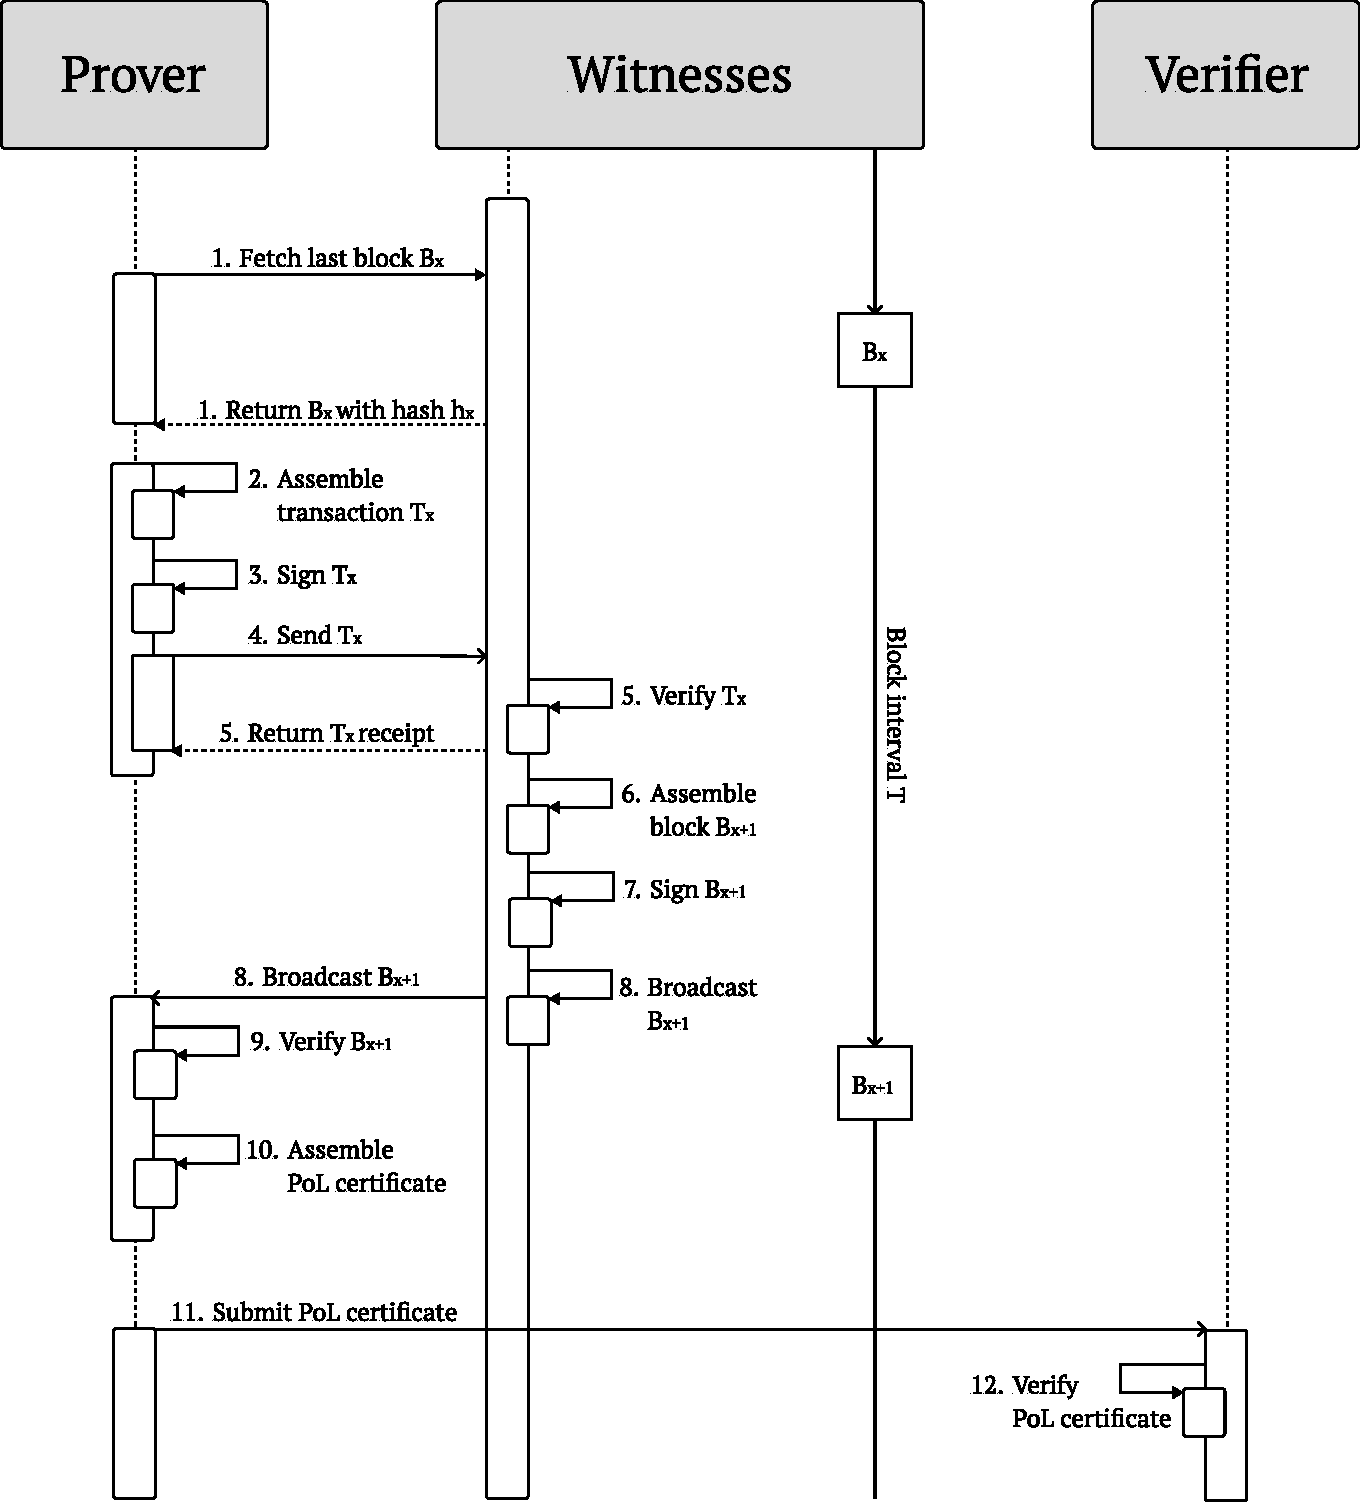
\includegraphics[width=\textwidth]{overview-pol-rel-seq.pdf}
    \caption{Sequence diagram overview of the proof generation process.}
    \vspace{-0.5cm}
    \label{fig:proof-of-location-overview-relative-pol-seq}
    \end{center}
\end{figure}

Up to this point, the protocol has been described in a relative manner, i.e., the prover is able to prove its location relative to the witnesses. The underlying mesh network enabled the short-ranged communication, while a permissionless consensus mechanism allowed for the time synchronization and generation of a verifiable certificate. The next section will provide a rough outline of how this protocol can be extended to achieve Absolute \pol{}, involving the introduction of verified space and time references.

\newpage

\subsection{Absolute \pol{}} \label{sec:protocol-fundamentals-abs-pol}

Having established a means for Relative \pol{}, ensuring space and time synchronization within a zone, the next step would be to extend the protocol to finally achieve Absolute \pol{}. A possible path consists in combining the procedure with a Global Time Synchronization Protocol and a Global Positioning System, as illustrated in Figure~\ref{fig:proof-of-location-overview-absolute-pol}.

\begin{figure}[h!]
    \begin{center}
    \includegraphics[width=0.55\textwidth]{overview-pol-abs-pol.pdf}
    \caption{Achieving Absolute \pol{} by combining Relative \pol{} with a Global Time Synchronization Protocol and a Global Positioning System.}
    \label{fig:proof-of-location-overview-absolute-pol}
    \end{center}
\end{figure}

The goal is to produce a \pol{} certificate that is spatio-temporally sound, relative to the zone, but which can, as well, be spatially and temporally acknowledged by any other node outside the zone. This effort may require, for instance, a global timestamping server, or protocol that can assert a certain level of globally secure timestamp accuracy in a tamper-proof manner. In a decentralized fashion, one example of such a system is a public Blockchain network, such as Bitcoin \cite{nakamoto2008bitcoin}, or Ethereum \cite{buterin2014next}. The same applies to the Global Positioning System (GPS). A standard system of geographic coordinates could be validated and embedded into the \pol{} certificate, to globally assert the location of the whole zone \cite{amoretti2018blockchain ,nosouhi2020blockchain}. It is worth noting that the Relative \pol{} protocol is flexible enough to accommodate any kind of higher level protocol, including more complex certificate formats, tighter trust levels, and composite information to be signed. This and further extensions are left for future work. \\

This chapter has laid the path towards a decentralized \pol{} protocol. We have started by proposing a mesh network topology to provide a decentralized and self-organizing network infrastructure. This underlying arrangement of nodes enables peer-to-peer and short-range communication, which is essential for the soundness of the protocol. Next, we have proposed a new way of synchronizing the internal clocks of trustless witnesses. This approach takes advantage of permissionless consensus mechanisms to establish zone-relative time consciousness and simultaneously enable the serialization of events in a tamper-proof manner. We have also considered the choice of a Turing-complete consensus system to allow for the decentralized execution of computations and deployment of zone-relative location services. Finally, we have proposed a \pol{} protocol that can produce a verifiable and spatio-temporally sound location certificate, relative to a zone. From Relative \pol{}, we are concluding the chapter with some thoughts on extending the protocol to achieve Absolute \pol{}.


\newpage
\section{Proof-of-Concept} \label{sec:proof-of-concept}

Esse do proident duis minim esse aute ut reprehenderit sint ut minim. Tempor exercitation aliqua occaecat eiusmod aliquip aute nostrud amet. Aliqua non commodo anim ex pariatur. Tempor consectetur veniam amet cupidatat excepteur. In aliquip voluptate esse non ullamco consectetur ut. Exercitation qui excepteur veniam fugiat commodo ex labore Lorem proident et sunt proident. Mollit est sit adipisicing consequat deserunt voluptate exercitation deserunt elit ut ad.

Est aute laborum minim officia aliquip dolor ut laboris proident quis eu officia quis culpa. Fugiat et ullamco velit veniam voluptate aute. Mollit pariatur magna fugiat ipsum voluptate exercitation mollit enim. Id sunt fugiat adipisicing labore exercitation magna commodo ex. Velit commodo culpa tempor mollit adipisicing qui eiusmod voluptate est veniam mollit occaecat. Culpa officia ad mollit in sit minim nulla aliqua ullamco.

\subsection{Infrastructure} \label{sec:proof-of-concept-infrastructure}

Minding to meet the requirements established in Chapter~\ref{sec:protocol-fundamentals}, the system design process and infrastructure choices for accomplishing the establishment of a Mesh Network were crucial in ensuring its operability. The following sections describe the designing of the system and the testbed setup, as well as the challenges faced during the establishment of the network infrastructure.

\subsubsection{System Design} \label{sec:infrastructure}

One of the critical decisions was the selection of an appropriate operating system (OS) for configuring and enabling an ad-hoc and dynamic Mesh Network. Multiple Linux distributions were initially explored, including OpenWRT, Raspbian, Ubuntu, and others. After careful consideration and a handful of failed attempts, OpenWRT lead the track to host the protocol implementation. OpenWRT's automated build tools and configurable packages, including the straightforward \emph{batman-adv} kernel module integration, load, and setup, made it a suitable choice for the high level flexibility and customization of the mesh metwork. The OS's active development community and extensive documentation further supported its use. As mentioned in Section~\ref{sec:background-wireless-mesh-networks}, OpenWRT is a lightweight solution for embedded devices, supporting a considerable set of platforms and toolchains for targetted integration of embedded software. Its choice turned out to be strategic regarding as well the role played in the spawning of decentralized and community-driven computer networks, powered by and actively contributing to such open source projects, all around the world\footnote{\url{https://en.wikipedia.org/w/index.php?title=Freifunk}}.

The OpenWRT image building process took advantage of the official Image Builder pre-compiled environment in order to create a custom image, skipping the need for source compilation\footnote{\url{https://openwrt.org/docs/guide-user/additional-software/imagebuilder}}. The image building process was automated with the help of a \emph{Dockerfile}, not only to allow for an easy integration and further testing of the mesh network related pre-compiled packages, but also to enable the experimentation with different network settings and the quick embedding and deployment of the \pol{} protocol software. The packages were chosen to provide deployment and debugging support for mesh networking using \emph{batman-adv}, wireless security using WPA/WPA2, working with the \emph{ext4} file system, and interacting with an Ethereum network via the official \emph{geth} client. The images were experimentally compiled for \emph{x86-64}, \emph{bcm27xx-bcm2708}, and \emph{bcm27xx-bcm2709} targets, being the last two ideal for the Raspberry Pi Zero and Raspberry Pi 2/3/4 models, respectively\footnote{\url{https://firmware-selector.openwrt.org/}}.

\subsubsection{Testbed Setup} \label{sec:infrastructure:testbed}

% Raspberry Pi failure deploymment
% Choice for QEMU for ease of testing and deployment
% Description of the testbed, including the hardware emulated, characteristics, etc.
% Description of the tap and bridge interfaces, etc.

The next step was to set up a testing environment for the deployment and running of the \pol{} protocol. Up to the delivery of this thesis, efforts are being made to port the generated OpenWRT image and compiled protocol modules to physical Raspberry Pis. However, the deployment on physical devices and the configuration of wireless interfaces is proving to be a challenge on multiple levels. The current drawbacks being faced are related to the automated enabling of the \emph{batman-adv} kernel module, in order to allow for the autonomous start of a dynamic and ad-hoc mesh network. Nevertheless, even when manually configuring the interfaces, the protocol process of dynamic neighourhood discovery is also failing, as the wireless interfaces are not able to easily detect each other, or establish a stable connection. Further investigations are being made to identify the root cause of these problems, and to finally uncover the solution for the deployment of the protocol on physical devices. These attempts and the physical demonstration of the \pol{} protocol are set for future work.

Meanwhile, to ease such development and testing hustle and to allow for a more flexible and faster deployment of the protocol, a virtualized environment was set up using QEMU (see Section~\ref{sec:background-wireless-mesh-networks}). The environment was configured to emulate a set of \emph{x86-64} target devices, and to run the OpenWRT image with the embedded and target-compiled \pol{} software. The testbed setup followed the guidelines of the official \emph{batman-adv} documentation\footnote{\url{https://www.open-mesh.org/doc/devtools/Emulation_Environment.html}}. The automated script expects the previously built OpenWRT image, and defines variables for the instance type, either "witness" or "prover", the instance number, and a GDB port number, for kernel debugging. The script creates a shared bridge for the cluster and a unique tap interface for each virtual machine, assigning to them an individual MAC address. Finally, the script launches QEMU by creating a new virtual disk image, as a copy-on-write snapshot of the OpenWRT image, and by setting up each virtual machine with 1GB of memory, 2 virtual CPUs, and a virtual SCSI disk. It assigns, as well, network interfaces to the instances. One uses the previously created tap interface to flush the mesh network traffic, and a second one is a virtual NIC to allow for the usual internet connection\footnote{\url{https://www.open-mesh.org/doc/devtools/OpenWrt_in_QEMU.html}}. KVM is also enabled in order to speed up the emulation, as well, a virtual RNG (Random Number Generator) and a virtual serial port. Up and running, with three witnesses and a prover instance, the testbed looks as depicted in Figure~\ref{fig:infrastructure:testbed}.

\begin{figure}[h!]
    \begin{center}
    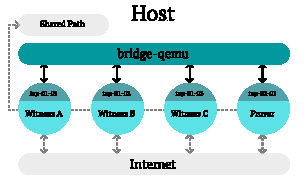
\includegraphics[width=0.9\textwidth]{proof-of-concept-qemu.pdf}
    \caption{Testbed setup for the \pol{} protocol.}
    \label{fig:infrastructure:testbed}
    \end{center}
\end{figure}

\subsubsection{Network Architecture} \label{sec:infrastructure:network-architecture}

After the establishment of the testbed, the physical networking layer is emulated by the bridge interface, which is set to pool all the mesh traffic that flows into and from the tap interfarces. The step that follows is the configuration of the \emph{batman-adv} kernel module, responsible for the dynamic and ad-hoc mesh network creation. This step was automated at the OpenWRT image building process, with the inclusion of custom instructions in the image startup scripts. These instructions set the routing algorithm and add the virtual Ethernet interface eth0, corresponding to the tap interface created before, to the batman-adv interface bat0. The interval time between the broadcasting of neighourhood discovery messages is set to 5 seconds, which determines how often a node should broadcast its presence in the network, and the bridge loop avoidance mechanism is activated, penalising the routing of traffic through routes with more hops. This last step is important to avoid the creation of loops in the network and to ensure that the traffic is always routed through the shortest path, i.e., forcing the nodes to communicate directly with each other, within the testbed. Finally, the script disables the firewall to avoid any interference with batman-adv, and flushes the IP addresses of both the eth0 and bat0 interfaces.

Subnetting is then done via the assignment an IP address to the bat0 interface. The IP address of each instance is generated based on the MAC address of the network interface eth0, establishing a non-conflicting address in the 192.168.0.x/24 subnet. After this step, the network is ready to use the TCP/IP protocol stack, and the \pol{} protocol can be deployed, configured, and run. The final network topology is depicted in Figure~\ref{fig:infrastructure:network-architecture}.

\begin{figure}[h!]
    \begin{center}
    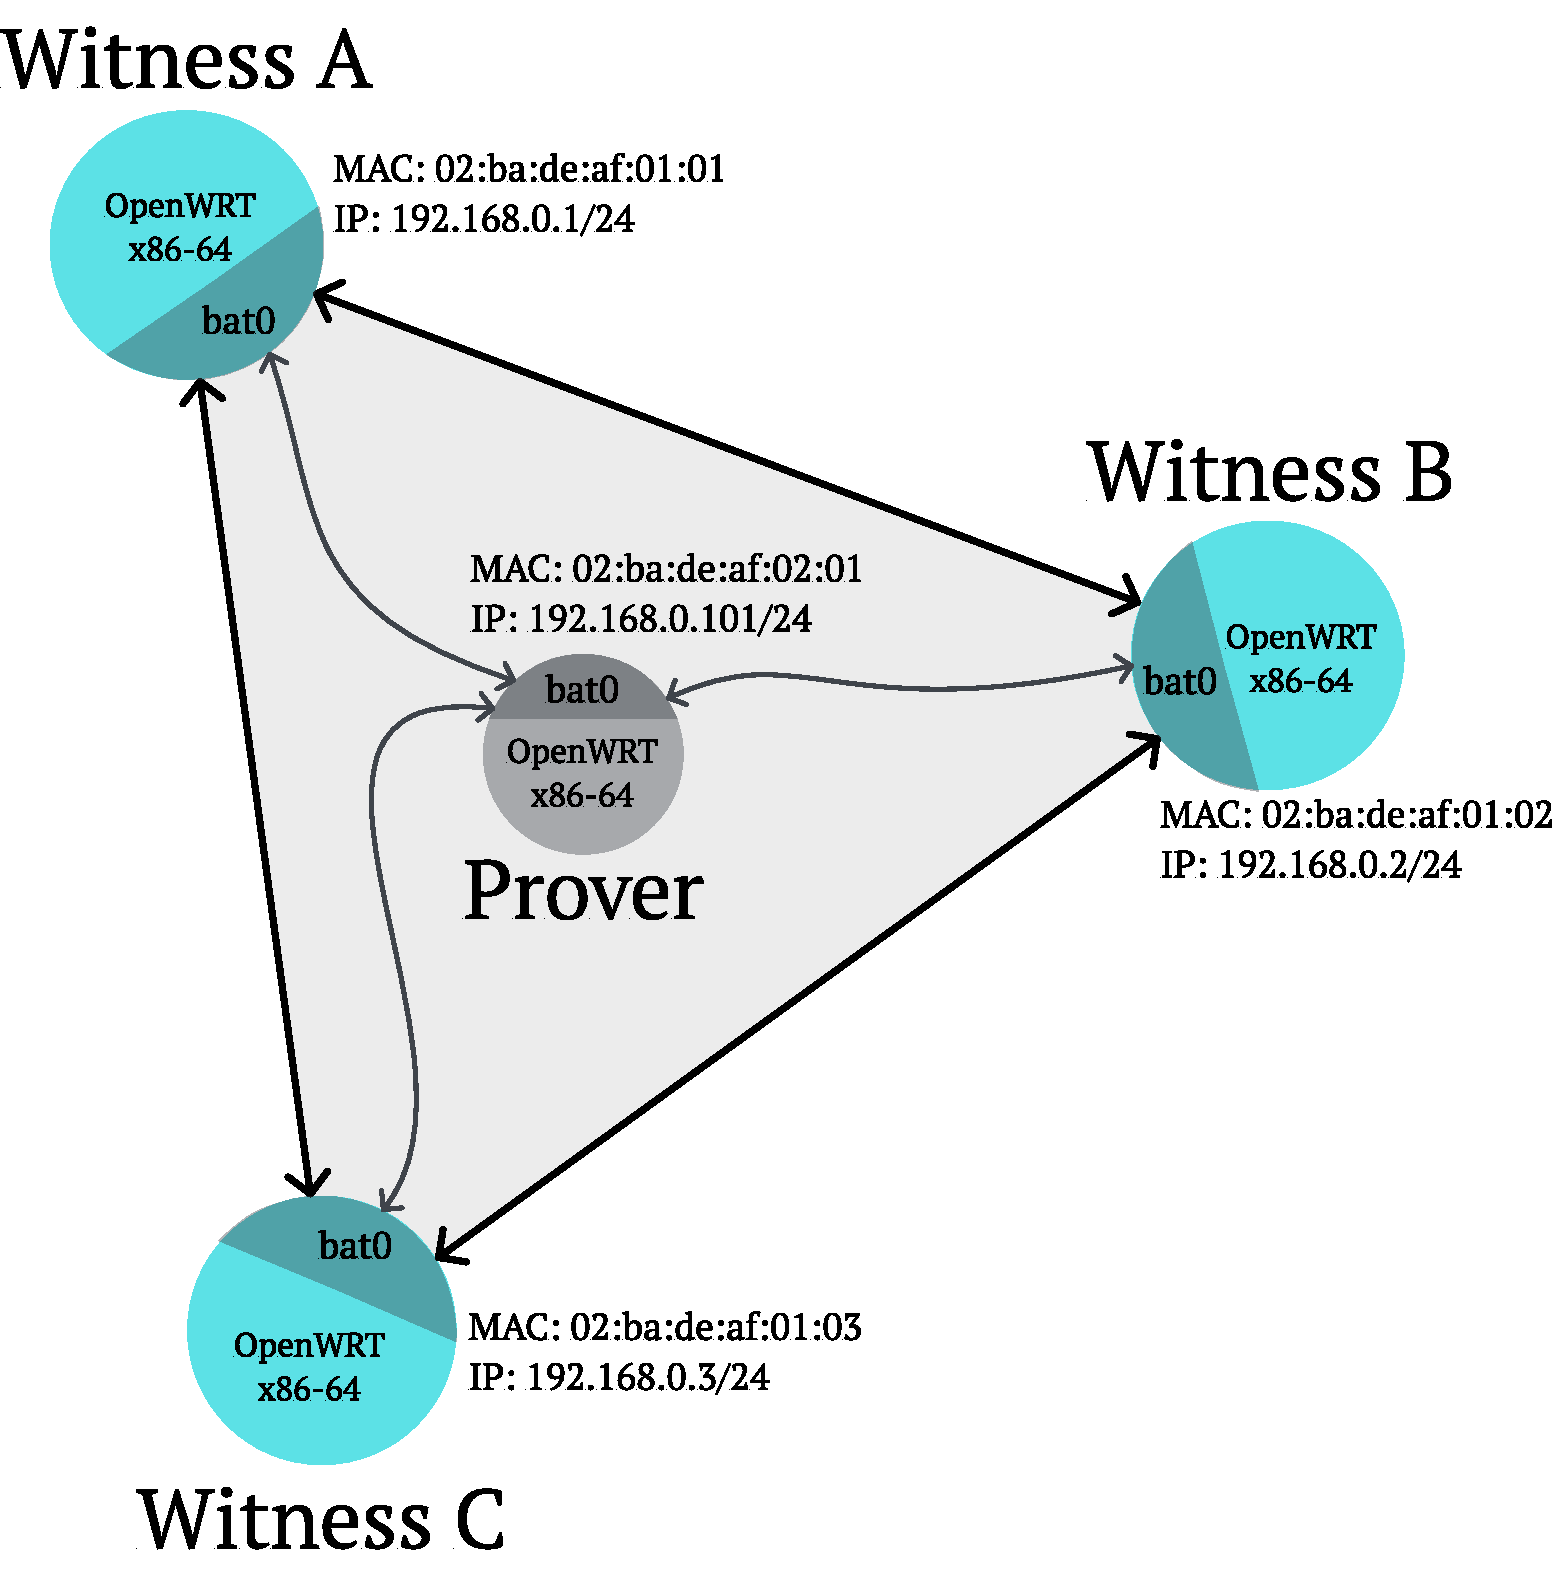
\includegraphics[width=0.7\textwidth]{proof-of-concept-network-topology.pdf}
    \caption{Network topology of the system under test, after configuring the \emph{batman-adv} interface and assigning IP addresses to the instances.}
    \label{fig:infrastructure:network-architecture}
    \end{center}
\end{figure}

\subsection{Protocol Implementation} \label{sec:proof-of-concept-pol-implementation}

The steps above ensured the emulation and establishment of the physical, data link, network, and transport layers, drawing up the foundation for the application layer, featuring the actual implementation of the \pol{} protocol. In this section, a description of the protocol setup is provided, including the reasoning and choice for the Blockchain framework to use. The processes of proof generation and verification are also detailed.

\subsubsection{Practical Permissionless Consensus} \label{sec:pol-implementation:practical-permissionless-consensus}

The outline provided in Section~\ref{sec:protocol-fundamentals-clock} identified the need for a clock synchronization mechanism that would finally enable spatio-temporal soundness. Space synchrony is achieved with the assumptions around the short-range communication means used by the protocol entities. Time synchrony, on the other hand, is achieved with a clock synchronization mechanism. The hypothesis constructed in Section~\ref{sec:protocol-fundamentals-clock} involved the employment of a permissionless consensus protocol to establish zone-relative time consciousness, but with the added benefit of providing strongly consistent serialization of transactions and total order of multidimensional events, instead of simply counting time in a unidimensional manner, via a plain clock synchronization protocol. The practicalities of employing a permissionless consensus mechanism involved the experimentation with a Blockchain framework, the deployment of an interacting client, and the setup of the network.

The beginning of the exploration process included the prototyping of an ad hoc Proof-of-Work based consensus protocol, to assess the feasibility of the hypothesis. This work was part of the 2022 Fall Semester's edition of the Distributed Systems seminar, where an analytical approach was taken to survey and evaluate multiple permissionless consensus mechanisms, pointing out the challenges of porting such protocols to resource constrained environments\footnote{\url{https://github.com/edurbrito/dist-sys-seminar}}. The results of the experiment were sufficiently encouraging to warrant the development or choice of a more robust and scalable implementation. Multiple open source projects were considered, and the ultimate decision relied on Ethereum and its flexible tooling for creating private networks\footnote{\url{https://geth.ethereum.org/docs/fundamentals/private-network}}. Its official client implementation, \emph{geth}\footnote{\url{https://github.com/ethereum/go-ethereum}}, was successfully blended into the OpenWrt image and each individual node got assigned both a private key and a public address, during startup.

The prerequisites for the establishment of an ad hoc Ethereum network expect first the configuration of a \emph{Genesis} file and a local data directory, to set the initial state of the network and progressively save the history, as the blocks get mined. Configuring the Genesis block resorts, as well, to the choice of a consensus protocol. The \emph{geth} client supports two main consensus protocols, a Proof-of-Work (PoW) and a Proof-of-Authority (PoA) based mechanism. Both protocols were tried out, but PoA was ultimately chosen for carrying out the remaining tests, as it offered a more controlled environment for the flexible adjustment of multiple parameters, such as the block time. A more thorough analysis of the PoW and PoA protocols, as well as trade-offs and performance comparisons, are left for future work. The PoA protocol relies on a list of authorized signers, which are allowed to mine blocks \cite{clique-eth}. The signers' list is defined in the Genesis block, and the private key of each signer is used to sign the blocks. The key pair generation was automated at startup and multiple utility programs were developed to facilitate the deployment of the nodes and the execution of the protocol. These custom programs were written in Golang and compiled for the target platform, to be used as part of the OpenWrt image, serving also as demonstration of the feasibility of the process of embedding new software into the image. The programs, among other tasks, automate the initialization of the Blockchain nodes, via the Genesis file, and the establishment of the network, via the discovery of bootnodes and connection of new peers. Each node exposes the necessary API endpoints to allow for the interaction with the rest of the protocol participants. Network rules were also configured to restrict the communication to the zone subnet, as well as a caching policy to avoid unnecessary resource consumption. Everything was accomplished with the help of the Ethereum \emph{geth} client and the final Blockchain network arrangement is illustrated in Figure~\ref{fig:pol-implementation:blockchain-network}.

\begin{figure}[h!]
    \begin{center}
    \includegraphics[width=0.75\textwidth]{proof-of-concept-blockchain.pdf}
    \caption{The Blockchain network setup.}
    \label{fig:pol-implementation:blockchain-network}
    \end{center}
\end{figure}

\subsubsection{Proof Generation} \label{sec:pol-implementation:proof-generation}

\subsubsection{Proof Verification} \label{sec:pol-implementation:proof-verification}


% Geth choice for the Ethereum client
% Geth setup, including the genesis block, clique PoA vs PoW, etc.
% Geth run
% Prover client, requests, smart contract deployment failure, etc.
% Verifier example



\subsection{Measurements} \label{sec:proof-of-concept-results}

Along with the implementation of the proof-of-concept, multiple experiments were conducted to evaluate the networking and computational performance of the proposed approach. The testbed was empirically hosted on a laptop with an AMD Ryzen 7 4700U CPU and 16 GB of RAM, running an x86-64 Linux 6.1.24-1-lts system. Every instance got assigned 1 GB of RAM and 2 virtual CPUs. 

The bridge interface, pooling all the mesh traffic exchanged between the tap interfaces, was the starting point for the networking measurements. All these interfaces had a maximum virtual bandwidth of 10 Mbit per second, assigned by the hosting system. The traffic was monitored using Wireshark\footnote{\url{https://www.wireshark.org/}}, and the metrics were collected throughout the various stages of the experiment, by listening to packets of different kinds, flowing through the bridge interface. Establishing the mesh network connectivity, the Ethernet frames belonging to the batman-adv protocol sized an average of 74 bytes, and the IPv4 related packets averaged at 278 bytes, presenting both protocols a seemingly linear throughput increase with the increase in the number of instances, as shown in Figure~\ref{fig:mesh-traffic}. 

\begin{figure} [h!]
    \centering
    \begin{subfigure}[b]{0.49\textwidth}
        \centering
        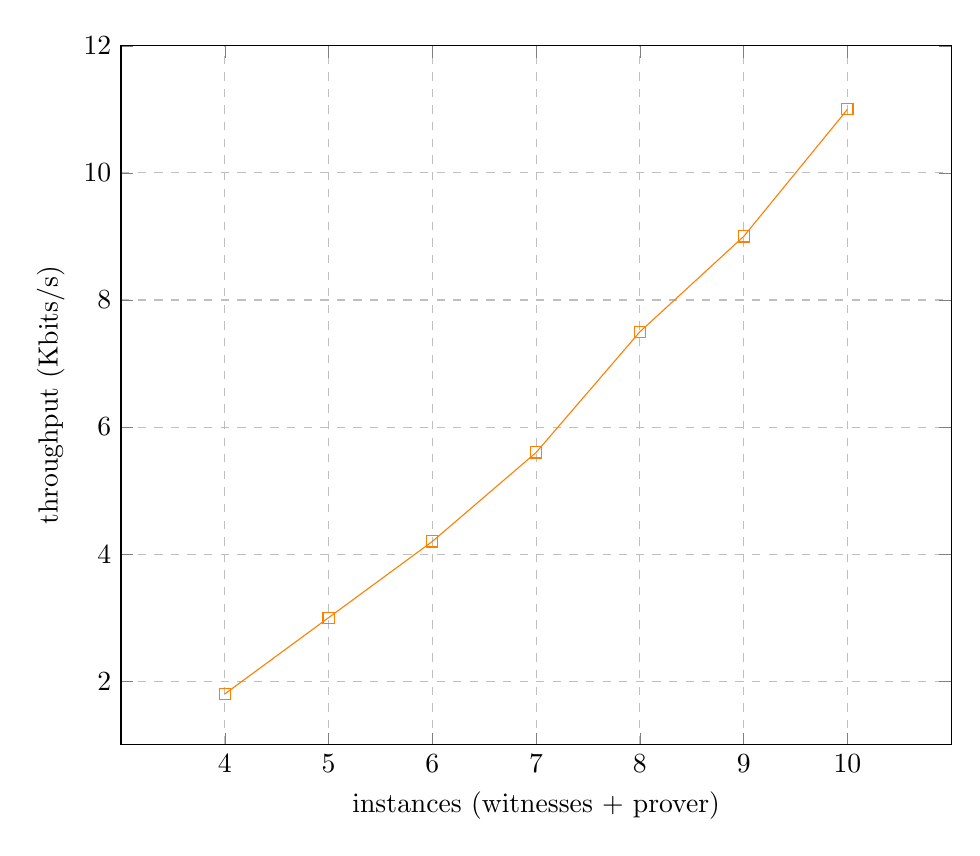
\begin{tikzpicture}
            \definecolor{line-color}{RGB}{92,255,230}
            \definecolor{line-color2}{RGB}{3,150,156}
            \begin{axis}[
                legend pos=outer north east,
                xlabel=instances (witnesses + prover),
                ylabel=throughput (Kbits/s),
                xmin=3, xmax=11,
                ymin=1, ymax=12,
                xtick={4,5,6,7,8,9,10},
                ytick={2, 4, 6, 8, 10, 12},
                grid=major,
                grid style={dashed},
                width=\textwidth
            ]
            
            \addplot[color=orange,mark=square] coordinates {
                (4,1.8) (5,3.0) (6,4.2) (7,5.6) (8,7.5) (9,9.0) (10,11)
                % (4,3.4) (5,5.7) (6,8.1) (7,11.2) (8,14) (9,16.8) (10,20)
            };
            \end{axis}
        \end{tikzpicture}
        \caption{Batman-adv traffic throughput.}
        \label{fig:y equals x}
    \end{subfigure}
    \hfill
    \begin{subfigure}[b]{0.49\textwidth}
        \centering
        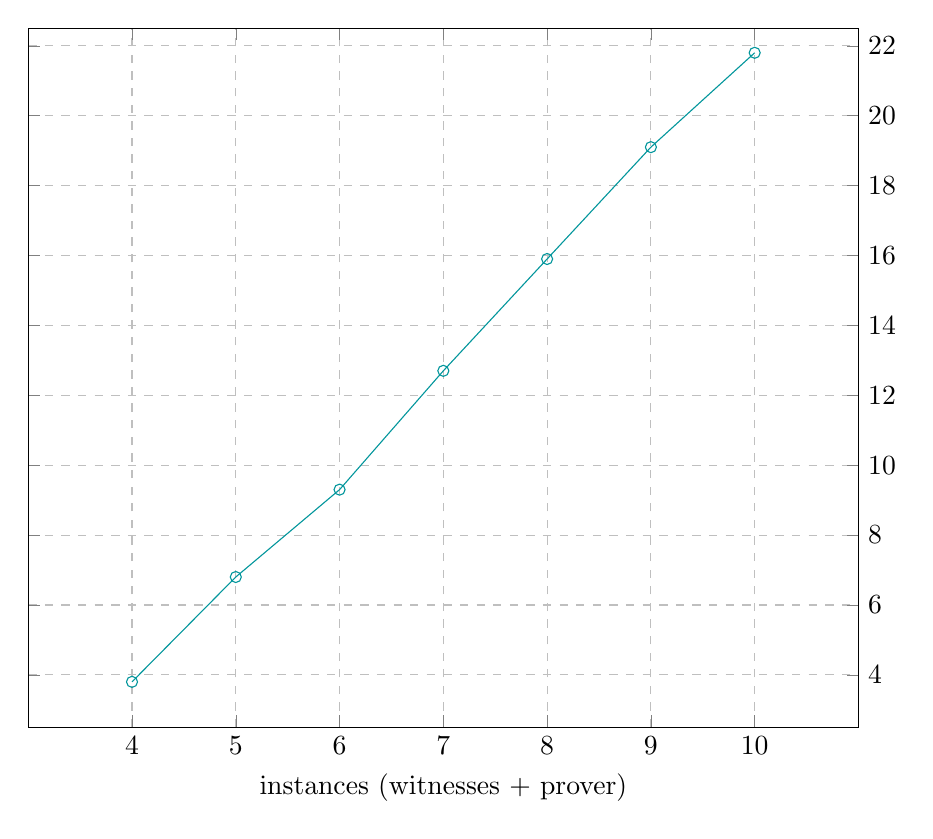
\begin{tikzpicture}
            \definecolor{line-color}{RGB}{92,255,230}
            \definecolor{line-color2}{RGB}{3,150,156}
            \begin{axis}[
                legend pos=outer north east,
                xlabel=instances (witnesses + prover),
                % ylabel=throughput (Kbits/s),
                yticklabel pos=right,
                xmin=3, xmax=11,
                ymin=2.5, ymax=22.5,
                xtick={4,5,6,7,8,9,10},
                ytick={2, 4, 6, 8, 10, 12, 14, 16, 18, 20, 22},
                grid=major,
                grid style={dashed},
                width=\textwidth,
            ]
            
            \addplot[color=line-color2,mark=o] coordinates {
                (4,3.8) (5,6.8) (6,9.3) (7,12.7) (8,15.9) (9,19.1) (10,21.8)
            };        
            \end{axis}
        \end{tikzpicture}
        \caption{IPv4 traffic throughput.}
        \label{fig:three sin x}
    \end{subfigure}
    \caption{Average protocol throughput, measured on the bridge interface.}
    \label{fig:mesh-traffic}
\end{figure}

The Blockchain activity was also monitored, in order to observe the protocol behaviour, regarding the block generation and proposal phases. Figure~\ref{fig:blockchain-blocks-generation} captures the number of messages exchanged between the instances, during a time frame of typical protocol activity. The interval time between blocks, set to 10 seconds, corresponds to the higher peaks of TCP traffic, while the UDP traffic is more evenly distributed.

\begin{figure}[h!]
\pgfplotstableread[col sep=comma]{data/blockchain-blocks-generation.csv}\datatable

\begin{tikzpicture}
    \definecolor{line-color}{RGB}{3,150,156}
    \definecolor{line-color2}{RGB}{167,169,172}
    \begin{axis}[
        xlabel=time (s),
        ylabel=messages,
        xmin=-2, xmax=102,
        ymin=-50, ymax=300,
        ytick={0, 50, 100, 150, 200, 250, 300},
        grid=major,
        grid style={dashed},
        width=\textwidth,
        height=0.5\textwidth,
        legend pos=north west
    ]

    \addplot[mark=*,line-color] table[x=x,y=TCP]{\datatable};
    \addplot[mark=+,line-color2] table[x=x,y=UDP]{\datatable};
    \addplot[mark=o,red] table[x=x,y=Batman-adv-orig]{\datatable};

    \legend{TCP, UDP, Batman-adv-orig}

    \end{axis}
\end{tikzpicture}
\caption{The network activity, with a block time of 10 seconds.}
\label{fig:blockchain-blocks-generation}
\end{figure}

Both CPU and RAM usage were also continuously measured across the whole experiment. The two virtual cores of each instance saw the CPU usage averaging at 2\%, peaking at 20\% when a witness would interact with the prover, in order to produce a \pol{} certificate. The overall RAM usage did not go beyond 200 MB. These numbers are in line with the expected behaviour of the protocol, running the PoA consensus algorithm, as a lightweight mechanism that may not require much computational power, suitable and adaptable to resource-constrained environments. The PoW consensus algorithm, on the other hand, would require a much higher and variable computational power, that would be difficult to predict and control, as it is not only manually configured, but dependent, as well, on the dynamic difficulty adjustment mechanism, in order to meet a fixed block time.

\TODO{I am thinking of completing one more experiment: Changing the block time interval and measure the failure rate of the generation of \pol{} certificates... This would show the effect of the block time on tackling the proxy attacks. What do you think? It shall result in an inverse relationship between the block time and the failure rate of the \pol{} certificates. The higher the block time, the lower the failure rate.}

% \begin{figure}[h!]
%     \begin{center}
% \begin{tikzpicture}
%     \definecolor{line-color}{RGB}{92,255,230}
%     \definecolor{line-color2}{RGB}{3,150,156}
%     \begin{axis}[
%         legend pos=outer north east,
%         xlabel=number of instances (witnesses + prover),
%         ylabel=throughput (Kbits/s),
%         xmin=3, xmax=11,
%         ymin=1, ymax=12,
%         xtick={4,5,6,7,8,9,10},
%         ytick={2, 4, 6, 8, 10, 12},
%         grid=major,
%         grid style={dashed},
%         width=0.8\textwidth,
%         height=0.4\textwidth,
%     ]
    
%     \addplot[color=orange,mark=square] coordinates {
%         (4,1.8) (5,3.0) (6,4.2) (7,5.6) (8,7.5) (9,9.0) (10,11)
%         % (4,3.4) (5,5.7) (6,8.1) (7,11.2) (8,14) (9,16.8) (10,20)
%     };
%     % \addlegendentry{batman-adv}

%     % \addplot[color=line-color2,mark=o] coordinates {
%     %     (4,4.5) (5,6.8) (6,9.3) (7,12.7) (8,15.9) (9,19.1) (10,21.8)
%     % };
%     % \addlegendentry{IPv4}

%     \end{axis}
% \end{tikzpicture}
% \caption{Average batman-adv traffic throughput, measured on the bridge interface.}
% \label{fig:mesh-traffic}
% \end{center}
% \end{figure}

% \begin{figure}[h!]
%     \begin{center}
% \begin{tikzpicture}
%     \definecolor{line-color}{RGB}{92,255,230}
%     \definecolor{line-color2}{RGB}{3,150,156}
%     \begin{axis}[
%         legend pos=outer north east,
%         xlabel=number of instances (witnesses + prover),
%         ylabel=throughput (Kbits/s),
%         xmin=3, xmax=11,
%         ymin=2.5, ymax=22.5,
%         xtick={4,5,6,7,8,9,10},
%         ytick={2, 4, 6, 8, 10, 12, 14, 16, 18, 20, 22},
%         grid=major,
%         grid style={dashed},
%         width=0.8\textwidth,
%         height=0.4\textwidth,
%     ]
    
%     \addplot[color=line-color2,mark=o] coordinates {
%         (4,4.5) (5,6.8) (6,9.3) (7,12.7) (8,15.9) (9,19.1) (10,21.8)
%     };
%     \addlegendentry{IPv4}

%     \end{axis}
% \end{tikzpicture}
% \caption{Average batman-adv traffic throughput, measured on the bridge interface.}
% \label{fig:mesh-traffic}
% \end{center}
% \end{figure}

% \begin{figure} [h!]
% \begin{tabular}{c c}
% \begin{minipage}{0.50\textwidth}
%     \begin{center}
%         \begin{tikzpicture}
%             \definecolor{line-color}{RGB}{92,255,230}
%             \definecolor{line-color2}{RGB}{3,150,156}
%             \begin{axis}[
%                 legend pos=outer north east,
%                 xlabel=instances (witnesses + prover),
%                 ylabel=throughput (Kbits/s),
%                 xmin=3, xmax=11,
%                 ymin=1, ymax=12,
%                 xtick={4,5,6,7,8,9,10},
%                 ytick={2, 4, 6, 8, 10, 12},
%                 grid=major,
%                 grid style={dashed},
%                 width=\textwidth,
%                 height=0.8\textwidth,
%             ]
            
%             \addplot[color=orange,mark=square] coordinates {
%                 (4,1.8) (5,3.0) (6,4.2) (7,5.6) (8,7.5) (9,9.0) (10,11)
%                 % (4,3.4) (5,5.7) (6,8.1) (7,11.2) (8,14) (9,16.8) (10,20)
%             };
%             \end{axis}
%         \end{tikzpicture}
%         \caption{(a) Average batman-adv traffic throughput.}
%         % \label{fig:mesh-traffic}
%         \end{center}
% \end{minipage}
% &
% \begin{minipage}{0.50\textwidth}

%     \begin{center}
%         \begin{tikzpicture}
%             \definecolor{line-color}{RGB}{92,255,230}
%             \definecolor{line-color2}{RGB}{3,150,156}
%             \begin{axis}[
%                 legend pos=outer north east,
%                 xlabel=instances (witnesses + prover),
%                 % ylabel=throughput (Kbits/s),
%                 xmin=3, xmax=11,
%                 ymin=2.5, ymax=22.5,
%                 xtick={4,5,6,7,8,9,10},
%                 ytick={2, 4, 6, 8, 10, 12, 14, 16, 18, 20, 22},
%                 grid=major,
%                 grid style={dashed},
%                 width=\textwidth,
%                 height=0.8\textwidth,
%             ]
            
%             \addplot[color=line-color2,mark=o] coordinates {
%                 (4,4.5) (5,6.8) (6,9.3) (7,12.7) (8,15.9) (9,19.1) (10,21.8)
%             };        
%             \end{axis}
%         \end{tikzpicture}
%         \caption{(a) Average IPv4 traffic throughput.}
%         \end{center}

% \end{minipage}
% \end{tabular}
% \caption{Example how to put two figures parallel to each other.}
% \label{fig:LCA_2_solutions}
% \end{figure}

% \begin{figure}[h!]
% \pgfplotstableread[col sep=comma]{data/br-qemu.csv}\datatable

% \begin{tikzpicture}
%     \definecolor{line-color}{RGB}{3,150,156}
%     \definecolor{line-color2}{RGB}{167,169,172}
%     \begin{axis}[
%         xlabel=time (s),
%         ylabel=throughput (Bits/s),
%         xmin=10, xmax=20,
%         ymin=-100, ymax=1300,
%         ytick={0,200,400,600,800,1000,1200},
%         grid=major,
%         grid style={dashed},
%         width=\textwidth,
%         height=0.5\textwidth,
%     ]

%     \addplot[mark=*,line-color2] table[x=Interval start,y=prover 1]{\datatable};
%     \addplot[mark=+,line-color] table[x=Interval start,y=witness 1]{\datatable};
%     \addplot[mark=x,line-color] table[x=Interval start,y=witness 2]{\datatable};
%     \addplot[mark=o,line-color] table[x=Interval start,y=witness 3]{\datatable};

%     \legend{prover, witness 1, witness 2, witness 3}

%     \end{axis}
% \end{tikzpicture}
% \caption{Ethernet traffic throughput, measured on the bridge interface.}
% \label{fig:mesh-traffic-3-witnesses}
% \end{figure}



% AMD Ryzen 7 4700U with Radeon Graphics (with SSE4.2)
% Linux 6.1.24-1-lts


\newpage

\section{Conclusion} \label{sec:conclusion}

The \pol{} problem was the main target of this thesis. Through theoretical and practical contributions, the problem was comprehensively dissected. The identification of the underlying concepts, hypotheses, and real-world applications was followed by a review of the state of the art, encompassing a wide range of trust levels and infrastructural scenarios. Inspired by previous work, this thesis delivered a novel approach to the problem. The proposed solution involved the specification of a decentralized \pol{} protocol and the implementation of a \poc{}. The final work mixes routing protocols for mobile ad hoc mesh networks and permissionless consensus mechanisms, in order to finally achieve collective agreement on one's presence in a specific location, at a certain point in time. The protocol was showcased in a distributed setting, featuring a modular network architecture that separates concerns between the different stages. The chosen technologies showed optimistic results that make the work suitable and adaptable to resource-constrained environments. The proposed protocol is a promising step towards achieving Absolute \pol{} in a decentralized and trustless manner.

The groundwork for the implementation of a novel \pol{} protocol has been established, but further investigation is still needed, for instance, to identify the most effective identity management systems and crypto-economic incentives to motivate nodes to collaborate and establish and maintain coverage zones, with the research on the processes of zone discovery and zone affinity management revealing to be essential for the overall success of the protocol. Another aspect that deserves further investigation is the shift from deterministic-finality Byzantine fault-tolerant algorithms to probabilistic finality consensus mechanisms. Formal verifications, measurements, and comparisons of the two approaches are necessary to determine the best candidates for decentralized \pol{}. Furthermore, this thesis has demonstrated the simplest case of applying a consensus mechanism to achieve time synchronization. Extending the approach to reach more accurate location attestations, making full use of the system's Turing Completeness for more complex logic, and ensuring the extensibility of the approach are all areas for future work. A thorough analysis of the robustness, security, privacy, and correctness of the baseline solution is also to be presented. The integration of privacy preserving mechanisms, such as zero-knowledge proofs, is also a point of interest. Ultimately, the deployment of the solution in physical devices and the evaluation of the performance in real-world scenarios is the missing step towards the full realization of the work.

\newpage

\subsection*{Acknowledgments}

The author would like to express gratitude towards his supervisors, for all the guidance, feedback, and support provided throughout the development of this thesis. All the people that have contributed to the reasoning and validation of the work are also acknowledged.

Words of appreciation should go, as well, to the multiple tools that aided the writing and development of this thesis. ChatGPT, Grammarly, Code Spell Checker, LTeX, and GitHub Copilot provided invaluable support throughout the working process. ChatGPT helped with summarizing, rephrasing, contextualizing, correcting, and paraphrasing indiscriminate sections of the writing content. Grammarly, Code Spell Checker, and LTeX provided grammar and writing suggestions, while GitHub Copilot facilitated pair programming and provided code and debugging support. Words of praise should also credit all the other tools, extensions, and development environments that, directly or indirectly, with or without AI features, contributed to the efficiency of the thesis development process.

% Measurements of the latency, throughput, etc. of the batman network
% Measurements of the latency, throughput, etc. of the Ethereum network
% Measurement of CPU usage, memory usage, etc. of the witness nodes
% Measurement of CPU usage, memory usage, etc. of the prover proof generation process
